\documentclass[a4paper, 11pt]{inte}

% Faire des marges un peu moins larges que celles par défaut
\usepackage[top=20mm, bottom=20mm, left=20mm, right=20mm]{geometry}
\usepackage[utf8]{inputenc} % Pour l'encodage 
% Reconnaître les caractères accentués dans les sources.
\usepackage[T1]{fontenc} 
% Meilleurs polices
%\usepackage{concmath}
\usepackage{fourier}
\usepackage[francais]{babel}
% Insertion d'images
\usepackage{graphicx}
% Pour le listing de code
\usepackage{listings}
\usepackage{color}
% Pour fixer l'interlignage
\usepackage{setspace} 
% Pour faire un index (ici glossaire)
\usepackage{makeidx}
% Pour gérer les liens internes et les URL cliquables
\usepackage{url}
% Pour les headers et footers
\usepackage{fancyhdr}
% Pour le logo en haut a droite
\usepackage{eso-pic} 
% Pour l'enroulement du texte autour des figures
\usepackage{wrapfig}
% Pour la couverture en PDF pleine page
\usepackage{pdfpages} 
% Pour la biblio bibtex
\usepackage{bibunits}
% Pour gérer les éléments flottants
\usepackage{float}
% Pour les cadres à ombrage du glossaire
\usepackage{fancybox}
% Pour faire des sous-figures correctement numérotées
\usepackage{subfigure}
% Pour mettre les liens cliquables
\usepackage{hyperref}
\usepackage{lettrine}
\usepackage{multicol}
\usepackage{rotating}
\usepackage{amsmath}
\include{pstricks}
\include{xcolor}


%headers, footers
\pagestyle{fancy}
\rhead{INSA de Lyon}
\lhead{Poly d'inté IF'2010}
\cfoot{\thepage}
\renewcommand{\footrulewidth}{0.4pt}

% Séparation entre les deux colonnes
\setlength{\columnsep}{0.8cm}
% Largeur de la ligne de séparation
%\setlength{\columnseprule}{1pt}

% Changer la fonte vers Helvetica
%\usepackage{helvet}
% Changer la fonte vers Libris ADF
%\usepackage{libris}
% Changer la fonte vers Venturis Sans
\usepackage[lf]{venturis}

% Pour mettre en sans-serif par défaut
\renewcommand*\familydefault{\sfdefault} 
% Unité pour pstricks
\setlength{\unitlength}{1mm}


% Couleur des url et des liens internes.

\definecolor{sectionColor}{rgb}{0,0,1}
\definecolor{subSectionColor}{rgb}{0,0,0.8}
\definecolor{subSubSectionColor}{rgb}{0,0,0.6}
\definecolor{coulcitation}{rgb}{0.90,0.90,0.90}
\definecolor{bleuLien}{rgb}{0, 0, 0.8}
\setlength{\headheight}{13.6pt}


\hypersetup{
    pdftitle={Poly d'inté IF'2010},    % title
    pdfauthor={Équipe d'inté IF'2010},     % author
    pdfsubject={On peut mettre plein de trucs ici. Alors la recette de la 	tarte à la rhubarbe : Pour 6 personne(s) -Pour la pate sablée : 300 g de farine, 2 cuillères à soupe d'huile, 2 cuillères à soupe de lait, 2 cuillères à soupe de sucre, 125 g de beurre mou, 1 jaune d'oeuf(conserver le blanc pour la crème) -Pour la garniture : une belle botte de rhubarbe pelée et coupée en gros dés , 2 cuillères à soupe de crème fraiche épaisse, 2 oeufs et le blanc restant, 125 g de sucre, un peu de lait ,1 cuillère à café de maïzena PREPARATION 1 Mélanger la farine, le sucre, le beurre ramolli, ajouter le jaune d'oeuf , l'huile et le lait. Malaxer, bien rajouter un peu de farine si nécessaire pour que la pâte ne colle plus aux doigts.  2 Placer la boule de pâte au frais, 1 heure environ.  3 Etaler la pate à la main dans un moule à manqué avec revêtement anti adhésif.  Disposer les tronçons de rhubarbe sur la pâte.  4 Dans un saladier, battre les oeufs plus le blanc avec le sucre, ajouter la maïzena, puis le lait et la crème en mélangeant bien. Garnir la tarte.  5 Cuire au four préchauffé à 225°C pendant 30 à 40 minutes, la crème ne doit plus être liquide.  6 La démouler une fois refroidie est risqué mais possible en utilisant 2 plats à tarte.  },   % subject of the document
    pdfkeywords={IF Inté 2010 -- Martius est un usurpateur qui n'a rien à faire là --. Oh, mais là aussi on peut marquer plein de truc. Alors si tu vois ça, tu peux envoyer un mail à l'équipe d'inté, ça nous fera plaisir d'être soutenu dans notre stupidité : \texttt{bonjourlesifs@gmail.com}.  Allez, à plus, et merci pour tout le poisson.}, % list of keywords
    colorlinks=true,
    linkcolor=bleuLien,          % color of internal links
    urlcolor=bleuLien, % color of external links
    linkbordercolor=bleuLien
}



\renewcommand{\LettrineFontHook}{\fontfamily{pag}%
                \fontseries{bx}\fontshape{it}\color{red}}

  \newenvironment{changemargin}[2]%
  {\begin{list}{}{%
    \setlength{\listparindent}{\parindent}%
    \setlength{\itemindent}{\parindent}%
    \setlength{\leftmargin}{#1}%
    \setlength{\rightmargin}{#2}%
  }\item }%
{\end{list}}


% Boites pour citation
\newsavebox{\auteurcitation}
\newsavebox{\boitecitation}
\newenvironment{citationi}[1]
{% 
    \savebox{\auteurcitation}{#1}
    \begin{lrbox}{\boitecitation}
    \begin{minipage}{.8\linewidth}
    \small \slshape «~\ignorespaces
}
{%
    \unskip{}~»  

    \par\nopagebreak\hfill\usebox{\auteurcitation}

    \end{minipage}
    \end{lrbox}

    \begin{center}
	\colorbox{coulcitation}{\usebox{\boitecitation}}
    \end{center}
}

\newenvironment{citationii}[1]
{% 
    \begin{lrbox}{\boitecitation}
    \begin{minipage}{.8\linewidth}
    \small \slshape «~\ignorespaces
}
{%
    \unskip{}~»  

    \end{minipage}
    \end{lrbox}

    \begin{center}
	\colorbox{coulcitation}{\usebox{\boitecitation}}
    \end{center}
}

\newcommand{\carre}[2]{%
\begin{center}
\begin{picture}(#1,#2)
    \framebox(#1,#2){}
\end{picture}
\end{center}
}

\newcommand{\orga}[1]{%
\begin{center}
	\includegraphics[height=5cm]{#1}%
\end{center}
}




\newcommand{\adresseCoupon}{%
\begin{center}
\colorbox{coulcitation}{
    \begin{minipage}{.8\linewidth}
	M\up{elle} Sandra \textsc{Mondain}\\
	Appartement 13 \\
	130, rue du 4 août 1789 \\
	69100 Villeurbanne 
    \end{minipage}
}
\end{center}%
}

\newcommand{\plex}[2]{%
    \vspace{0.3em}
    \shadowbox{#1} \\
    #2

}



\begin{document}
\tableofcontents
\begin{multicols}{2}
{
    \begin{center}
\footnotesize
Rédigé avec amour et attention par l'équipe d'inté IF'2010, en utilisant
\LaTeX{} et une bonne tripotée de logiciels libres. \\
\textbf{Rédaction : }Paul, Julien, Guillaume et d'autres.\\
\textbf{Mise en page : }Paul.\\
\textbf{Illustrations :} Nical.\\
\textbf{Page de couverture :} Étienne.\\
\textbf{Relecture :} Marc, Vincent.\\
\normalsize
\cc \ccby \ccnc \ccsa
\end{center}
}
\end{multicols}

\newpage
\begin{multicols}{2}
\section{Introduction}
    Aïe aïe aïe, ça y est tu as reçu la confirmation que l'année prochaine tu seras à l'INSA de Lyon, en département Informatique en plus...

\vspace{1em}

Laisse moi te dire que tu es sacrément -- suspense -- bien tombé(e) ! Alors
bienvenue dans ta nouvelle vie !


\vspace{1em}

Pour certains c'est l'occasion de changer d'environnement, d'entamer une
nouvelle page de sa vie,  d'autres connaissent déjà un peu la maison mais
ne savent pas vraiment où ils vont en ayant coché la case «~Département
Informatique~» en fin de deuxième année. Vous allez donc vous retrouver dans
une promo composée de gens d'origines variées, qui seront comme vous parachutés
dans cette nouvelle vie qu'est la vie d'étudiant à l'INSA de Lyon !


\vspace{1em}

Bien entendu les questions fusent... Comment ça va se passer l'année
prochaine ? Est-ce que je vais me retrouver tout seul ?  Est-ce que les gens
sont sympa ? Est-ce que  Lyon c'est bien ? Comment organiser mon arrivée du
mieux possible ? Est-ce que les loutres volent mieux au parc de la Feyssine
qu'au parc de la Tête d'or ?


\vspace{1em}

Toutes ces interrogations, aussi capitales soient-elles pour ton arrivée et ta
nouvelle scolarité, vont trouver réponse ici-même dans ce magnifique
«\texttt{polydintegration2010.pdf}» que tu viens d'ouvrir ! 


\vspace{1em}

Ainsi au travers de ces quelques pages, rédigées avec amour par tes futurs
hypothétiques parrains, nous allons te présenter non seulement l'organisation
de ta future (\emph{et géniale !}) nouvelle année, mais aussi toute ta première
semaine, la semaine d'intégration  !


\vspace{1em}

Et là, je vois tout autour de moi les visages pâlir, les gens se mettre à
trembler de peur, le ciel s'assombrit tout autour de vous, un orage se
déclenche, Céline Dion se remet à chanter, vous réalisez d'un coup : ça y est,
je vais être bizuté !


\vspace{1em}

Ce à quoi nous répondons :

\begin{citationi}{ \reflectbox{©}\emph{padenot} }
    Alors là, déjà, NON ! 
\end{citationi}

Après cette superbe citation, que vous aurez l'occasion d'entendre à de
nombreuses reprises, nous allons expliquer un peu ce que c'est que la «~semaine
d'intégration~».

On est tous passé par l'étape de devoir «~changer de vie~», devoir quitter notre
cocon familial, notre petit(e) FAC/IUT/Prépa , notre petite ville qu'on
connaissait si bien et en même temps qu'on connaissait trop.
Et maintenant, paf pastèque, ça arrive d'un coup, on va se retrouver parachuté
à Lyon et à l'INSA en plus, loin de cette «~petite ville qu'on aimait tant~»,
sans vraiment connaître grand monde...

Tout ça pour dire qu'on a tous à un moment ou à un autre été à votre place ...
du moins on se l'est tous imaginés, car ça c'était sans compter cette fameuse
semaine d'intégration que nos très chers parrains nous avaient préparée ! Grâce
à elle nous avons pu créer des liens forts entre nous et devenir la promo
soudée que vous allez rencontrer dès Septembre. Et pour chacun d'entre nous,
cela reste un souvenir d'une période excellente, un moment fort de notre
vie probablement !

Toutes les animations sont faîtes pour que vous puissiez rencontrer les
personnes qui deviendront peut-être d'excellents amis (\emph{nous c'est arrivé,
vous ça arrivera !}), vos futurs camarades de groupe (\emph{nous c'est
arrivé, vous ça arrivera !}), vos futurs binômes (\emph{je suis lourd
hein !}), et peut-être plus...

Alors rassurez vous, pas de bizutage avec nous, uniquement des jeux,
sorties, animations, soirées et un week end d'intégration de folie, qui
vous feront vous sentir chez vous dès les premières minutes de votre vie
insalienne.

Nous avons eu droit à ca l'année dernière, et devinez quoi : Notre objectif
cette année c'est de faire pareil pour vous ! Alors dévorez vite le poly afin
de découvrir à quelle sauce vous allez être mangés en septembre !

Il ne me reste qu'à vous souhaiter d'excellentes vacances et à vous donner
rendez vous dès la troisième semaine de Septembre !

Parce que nous, au nom de toute l'équipe : on vous attend avec impatience bande
de loutres !
\vspace{1cm}
\begin{flushright}
\emph{Juju, Resp'inté 2010}
\end{flushright}
\newpage

\section{Présentation du département}
    Bon, l'inté c'est bien, mais il faudrait d'abord commencer par connaître ce à quoi on s'intègre non ? 

Alors pour démarrer en douceur, voilà une petite présentation du département, histoire de savoir ce qui vous attend dès septembre ! 

    \subsection{Lieux importants}
    Dans cette partie, on va essayer de vous présenter les lieux phares de votre scolarité : 

\paragraph{Le département}
Situé à proximité du Grand Restaurant, et de l'arrêt de tram Gaston Berger
(Ligne T1), le département informatique se situe en réalité aux deuxième et
troisième étages du bâtiment Blaise Pascal, le premier étant occupé par le
département Sciences et Génie des Matériaux (vous les reconnaîtrez facilement :
ils sont toujours devant vous à la machine à café... ahem).

\vspace{1em}

Au deuxième étage, vous trouverez les salles de TP (5 salles Windows dont trois
avec des machines déportés, et une salle Linux) ainsi qu'une salle de
TD/TP où vous effectuerez les phases de conception des projets. Il est à noter que deux
salles Java Sun Spot sont aussi mises à disposition à cet étage. Tout
cela vous sera rappelé lors d'un TP de présentation en début d'année.

\vspace{1em}

Au troisième étage se trouvent les salles de TD : rien d'exceptionnel, ce sont
des salles avec des tables, des chaises, un tableau, et un ordinateur pour le
prof (car on est en informatique tout de même !).

\vspace{1em}

Chose importante, nous partageons aussi nos locaux avec plusieurs laboratoires
de recherche en informatique, nous sommes donc quasiment tout le temps en
contact avec les chercheurs du LIRIS\footnote{\url{http://liris.cnrs.fr/}}, entre autres, qui sont aussi pour certains
nos enseignants, et ça, c'est super pour ceux qui sont intéressés par ce domaine !

\paragraph{L'Amphi Gaston Berger}
Lieu culte, voire mythique, certaines légendes estudiantines racontent que l'on
y dispense des savoirs mystérieux en informatique... Malheureusement, le chemin reste
encore long pour... Ah, on me signale à l'oreillette qu'il s'agit en réalité de l'amphi où se
déroulent tous les cours magistraux qui vous seront donnés en 3 et 4 IF... Vous
allez donc y passer un certain nombre d'heures, alors courage ! 

\paragraph{Le bâtiment des Humanités}
Situé à mi-chemin entre le département et la Maison des Étudiants, c'est ici
que vous aurez tous vos cours de tout ce qui n'est pas informatique... C'est à
dire Sciences Humaines et Communication (SHC) et les langues vivantes. 
Ce bâtiment est le centre névralgique de l'activité culturelle à l'INSA, et il
est souvent le cadre d'expositions d'art sympathiques pour peu que l'on apprécie ce sujet !

\paragraph{Le Grand Restaurant}
Autre lieu important du campus, le Grand Restaurant de l'INSA, où vous
serez conviés à vous repaître tout au long de l'année ! La chose fourbe de l'histoire, c'est qu'il abrite en réalité un restaurant, surnommé le «~Beurk~» (vous verrez vite pourquoi), mais aussi
un snack, le Prévert, plus connu sous le nom de Pervert, qui s'avère
relativement pratique les midis/soirs où l'on a pas beaucoup de temps pour manger, mais ce
qui est servi est la plupart du temps «~un peu lourd à digérer~».

\vspace{1em}

À noter que deux autres restaurants universitaires sont présents juste à l'extérieur du campus et proposent des repas à l'unité. Utile pour les potentiels externes !

\paragraph{La Maison des Étudiants}
Lieu phare de l'INSA, ce bâtiment situé juste derrière celui des Humanités
abrite le coeur de l'associatif Insalien, c'est à dire le Bureau des Étudiants (ou
BdE), dont une rapide présentation vous est faîte un peu plus loin dans le
poly. Pour continuer dans le domaine associatif, le bâtiment contient le
club lecture (où vous trouverez une foison de bouquins/BD/mangas), un salon de
lecture/réunion et très prochainement une salle télé !
Ce bâtiment abrite aussi les deux autres restaurants de l'INSA :

\subparagraph{Le Grillon}
Restaurant qui illustre parfaitement la citation suivante «~\emph{Plus c'est long,
	   plus c'est bon !}~». N'y voyez aucun sous-entendu, c'est juste que ce qui est servi là-bas est probablement
ce que vous pourrez avoir de meilleur sur le campus. En revanche, ça se paye car le restaurant 
est généralement surchargé et il faut donc se munir de patience pour pouvoir y manger ! Avis aux gastronomes !

 \vspace{1em}
 
\subparagraph{L'Olivier}
Restaurant  spécialisé dans les «~pizza/pâtes~» et autres plats venus du fin
fond de l'Italie, on y accède un peu plus rapidement qu'au Grillon et on y
mange assez bien le plus souvent !

\paragraph{La K-Fêt}
Envie d'aller vous jeter un godet après une rude journée ? Envie d'aller
décompresser à la fin des partiels ? Ne cherchez plus : La K-Fêt est faite
pour vous !

\vspace{1em}

Lieu mythique des soirées Insaliennes, la K-Fêt se trouve dans le patio de
la maison des élèves. C'est le bar associatif de l'INSA, tenu par de courageux
étudiants volontaires !

\vspace{1em}

Elle vous assure boissons et bonne ambiance quasiment tous les soirs, et à
moindre coût !

\vspace{1em}

Le jeudi précédent chaque période de vacances, une «~Boom K-Fêt~» est organisée
pour fêter la fin des cours, soirées mémorables pour la majorité ! À ne
pas rater !

\vspace{1em}

À noter que l'équipe d'inté IF y sera en soirée pendant les 2 ou 3 jours qui
précèdent le début de vos cours, donc si vous voulez nous rencontrer et
accessoirement passer une bonne soirée, n'hésitez plus ! On sera de toute façon
facilement reconnaissables, et nos coordonnées vous sont données dans le
paragraphe Planning (page \pageref{rplanning}) du poly !

\paragraph{La Rotonde}
Et oui, sous ce nom se cache en réalité la salle de spectacles de l'INSA !
Entièrement gérée par une association d'étudiants, elle a une
capacité de 500 places, et se met à la disposition des autres associations, avec
des prestations techniques (lumières, décors...) dignes de ce nom !

\vspace{1em}

Ansi, toute l'année est ponctuée par différentes animations :
\begin{itemize}
\item  Séance cinéma : CinéClub
\item  Pièces de théâtre et matchs d'impro : TTI et section Théâtre-études
\item  Spectacle de Danse : section Danse-études
\item  Concerts Ziket : Section Musique-études / Association Musicale de l'INSA (AMI) 
\end{itemize}

\paragraph{Les logements}
Si tu es admis direct, sache que tu as toutes tes chances d'avoir un logement
dans l'une des nombreuses résidences de l'INSA. La qualité est plus que correcte,
mais quelques points peuvent jouer en défaveur de cette solution : la connexion internet, qui
permet de travailler, tout au plus (quand il y a
vent arrière), et l'obligation de manger matin, midi et soir aux
restaurants de l'INSA, ce qui pourrait en lasser certains à la longue (rassures-toi, jusqu'à présent personne n'en est mort).
Enfin, ne nous voilons pas la face, c'est quand même une excellente expérience,
et habiter à 1 minute 30 à pied du bâtiment IF et des restaurants du campus a certains avantages indéniables.

\vspace{1em}

Ces magnifiques oeuvres de l'architecture Insalienne se composent, pour la
grande majoritée, d'un sommier, d'un matelas (les draps, couvertures et
oreillers ne sont pas fournis), d'une ou deux plaques électriques, d'un frigo,
d'une douche, de toilettes, d'un bureau (plus ou moins grand selon la taille de la
chambre), de nombreuses prises de courant, d'une prise Ethernet (la
connexion se fait par VPN) et TV (câbles non fournis, mais
achetables au BdE si besoin), sans oublier les étagères (plus ou moins grandes
selon les chambres : les rangements en plastiques sont
un bon remplacement) et une chaise (de facture douteuse : mieux vaut prévoir de
s'acheter un bon gros fauteuil de bureau bien confortable !). C'est à peu près tout, et c'est déjà pas mal !

\vspace{1em}

Du côté de l'accueil, à ton arrivée dans la résidence, un responsable t'emmènera visiter ton
nouvel antre en échange du bon d'emménagement que tu auras préalablement
récupéré à la Direction Des Résidences. Après une visite expédiée aussi vite
qu'une lettre à la poste, tu es désormais chez toi (n'oublie pas de regarder
l'état des chauffages, lumières, volets, fenêtres,  etc. lors de la visite
avec le régisseur, on sait jamais...) !

\vspace{1em}

Te voilà maintenant dans ta nouvelle turne, à deux portes d'autres IFs, en entouré par de gentils étudiants !
N'hésite pas à faire connaissance avec le voisinage, on ne sait jamais quelle surprises il réserve !

    \subsection{Scolarité}
    \vspace{1em}
\begin{citationii}
\emph{L'INSA c'est bien beau, mais au final on y fait quoi ?}
\end{citationii}
Au final, tu t'es engagé à l'INSA, mais tu te poses, comme tous les autres, cette
question !
Pas de panique, tes supers parrains sont là pour y répondre !
La scolarité à l'INSA est basée sur un modèle d'université, c'est-à-dire cours
magistraux en amphi, Travaux Dirigés (TD) afin de garantir la compréhension des
cours et enfin Travaux Pratiques (TP) pour les appliquer.

\subsubsection{Amphis}
Les cours en IF se déroulent sous forme de cours magistraux d'une durée de
1h30, à raison de deux par matinée. Ils sont organisés en modules qui
seront traités de manière cohérente par la suite dans les TD/TP.

\vspace{1em}

La présence en cours est obligatoire, mais non vérifiée. Le meilleur conseil que
nous puissions te donner vis-à-vis de cela est que «~ce qui est fait n'est plus à
faire, et ce qui n'est pas fait reste toujours à faire~». En d'autres termes, les
amphis peuvent te permettre d'assimiler le bagage théorique assez rapidement, et
bien qu'il existe de nombreux moyens d'acquérir ce bagage, l'amphi, à
condition qu'il soit bien suivi et accompagné de prises de notes, reste le moyen le plus 
efficace (et de loin) ! Après tu sais probablement bien mieux que nous ce dont tu as besoin !
\subsubsection{TD}
Les TD t'occuperont deux après-midis sur les quatre de cours dans la semaine.
L'objectif ici est de mettre en pratique les cours de façon à mieux les
maîtriser, et c'est aussi l'occasion d'avoir un échange privilégié avec
l'enseignant pour pouvoir poser des questions. Les TD à l'INSA n'ont pas grand chose
de différent avec ceux que tu as déjà eu l'occasion d'avoir ! 

\vspace{1em}

Truc sympa, c'est que les profs, pour la grande majorité, ne voient aucun
inconvénient à ce que nous prenions des notes sur ordinateur. Pour
certaines matières c'est assez infaisable (nos meilleurs experts en \LaTeX{} se
sont brisés le nez en maths...), mais ça reste pratique. Toutefois les
amateurs du papier-crayon restent majoritaires.
\subsubsection{TP}
Les TP sont l'élément clé de l'enseignement en 3IF. En effet, ils
te donneront l'occasion d'appliquer le bagage de connaissances acquis dans
les cours et approfondi dans les TD. Deux séances de TP (de 4h chacune) sont
organisées par semaine.

\vspace{1em}

Ils peuvent être de formes multiples (TP papier, programmation, etc.)
    et de durée variable. Par exemple, certains sont à rendre en fin de séance,
    d'autres ont un délai de 5 semaines maximum à partir de la première séance (attention
	avec ces derniers, le délai accordé est souvent piégeur, et il ne faut pas s'y prendre à la dernière minute).
    
\vspace{1em}

Les TP sont aussi l'occasion d'apprendre le travail en équipe. En effet, pour toute la
3IF, tu travailleras en collaboration avec une autre personne (différente chaque trimestre) qui
sera ton binôme, et avec qui il faudra répartir la charge de travail.

\vspace{1em}

Tu l'auras compris, une des plus grosses difficultés de la 3IF est de réussir
à gérer correctement l'enchaînement des TP de façon à pouvoir tous les
traiter de manière suffisante, alors sois prévoyant si tu ne veux pas
exploser ton budget caféine et raccourcir drastiquement ton temps de sommeil ! (Avec
du recul, c'est un peu comme de l'ordonnancement de tâches sur un processeur double coeur...) 

\vspace{1em}

Un dernier point : attention à la sur-qualité, c'est de la non-qualité ! Voici un principe de
base en informatique, et on te le répètera bien assez souvent durant l'année !

    \subsection{Enseignements}
    En IF, on fait de l'informatique, certes, mais c'est quand même un domaine assez
large. Les matières étudiées en 3IF sont (en gros) :
\begin{itemize}
    \item La programmation (C, C++, Java).
    \item La conception (UML, Merise) et le génie logiciel.
    \item La gestion des données (SQL, XML, administration, algèbre relationnel).
    \item L'algorithmie (mathématiques discrètes, intelligence artificielle, imagerie numérique).
    \item L'architecture des ordinateurs.
    \item Les réseaux, les systèmes d'exploitation.
\end{itemize}

\vspace{1em}

L'accent est mis sur l'acquisition de méthodes et sur la généralité, pour savoir faire beaucoup
de choses différentes. Bien qu'il soit utile de connaître le \texttt{C++} ou le \texttt{SQL} sur le bout
des doigts, la notation ne se fait que rarement sur le code, et même si l'on pourrait croire au premier abord que les
DUT ont l'avantage, il n'en est rien au moment des résultats.

\vspace{1em}

Tout cela est complété par une bonne dose de cours de maths supplémentaires : probabilités,
traitement du signal, analyse numérique, qui trouveront toujours une application dans les TP.

\vspace{1em}

Concernant les DS, le début de l'année est plutôt calme, et les premiers
commencent assez tard. Certaines matières voient leur évaluation se
passer très tard dans l'année alors que le cours a été fait beaucoup plus tôt,
d'où l'intérêt de prendre efficacement des notes lors des amphis/TD, afin de ne
pas perdre son temps au moment des révisions.

\vspace{1em}

La charge de travail est assez irrégulière, et il est capital de bien s'organiser pour
pouvoir réussir au mieux et ne pas passer ses nuits à finir un TP. Un bon conseil : ne remets
jamais au lendemain ce que tu peux faire le jour même !

\newpage
\section{Planning de l'inté}\label{rplanning}
    Que tu viennes du PC (premier cycle de l'INSA), de DUT, de la fac, de CPGE ou
que tu sois là par hasard (ça arrive même aux meilleurs), cette période de
l'année vise à faire de toi un vrai 3IF. Le but de la semaine d'inté (et un peu plus) est de
faciliter les rencontres entre les gens de la promo. Bien entendu, rien n'est obligatoire, mais
tout est fait pour que tu passes du bon temps, donc si j'étais toi, je viendrai...

Si tu arrives plus tôt à l'INSA et que tu t'embêtes, tu peux contacter l'équipe d'inté d'à peu près plein de manières :
\begin{itemize}
      \item SMS/coup de fil au 06 27 36 91 36 (Paul)
      \item Email à \texttt{bonjourlesifs@gmail.com}
      \item Twitter : un petit message à \texttt{@bonjourlesifs}.
      \item Facebook sur la page du groupe BonjourLesIfs.
\end{itemize}

\vspace{0.5cm}

{
    \hspace{-2cm}
\begin{tabular}{cccc}
	
\includegraphics[height=2cm]{images/telPaulQRcode.png} & 
\includegraphics[height=2cm]{images/qrcodeBjrLesIfsTwitter.png} & 
\includegraphics[height=2cm]{images/qrcodeEmail.png} & 
\includegraphics[height=2cm]{images/qrcodeFacebook.png} \\
	Tel. & \href{http://twitter.com/bonjourlesifs}{Twitter} & Email &
	\href{http://www.facebook.com/group.php?gid=120929821278518}{Facebook}\\
\end{tabular}
}

\vspace{0.5cm}
N'hésite pas à utiliser tous ces moyens, au cas où l'on se soit endormis sur un planning orga. 

En attendant la semaine d'inté, tu peux tous les jours retrouver plein d'IFs sur
\url{http://bonjourlesifs.tumblr.com}, le fabuleux site mis en place par tes futurs orgas préférés.

    \subsection{Vendredi 10 : Découverte du départ'}
    La plupart des gens voient où se situe le depart', mais peu en ont déjà
vu les entrailles. Le but de cette journée est de te familiariser avec le
département IF : visite des lieux, première session glandouille en salle
détente (dans laquelle tu passeras beaucoup de temps !), premiers cafés ou
thés, tout en discutant avec les orgas présents et les autres bizuths.

\vspace{1em}

De 9h à 17h, on t'attend au rez-de-chaussée du bâtiment Blaise Pascal
(voir le plan, page \pageref{plan}).

    \subsection{Vendredi 10 : Soirée K-Fêt}
    Première soirée, première soirée K-Fêt. Une bonne occasion de discuter autour
d'une bière (ou autre),  de rencontrer des orgas, des 4IFs, et d'autres bizuths.
Rendez-vous aux alentours de 21h , à la K-Fêt (le bar associatif de l'INSA, à
côté de la Maison des Étudiants, et de la Rotonde, la salle de spectacle
du campus, de toute façon, tu peux le voir sur le plan).

    \subsection{Samedi 11 : Visite du campus}
    Bon nombre de personnes le connaissent déjà mais il faut aussi penser aux
autres, on te propose donc de visiter le campus en entier, et crois-nous il est
de taille assez respectable. Point relativement indispensable pour les admis direct,
généralement marrant pour les autres (qui ont forcément des anecdotes à
propos de certains lieux), on se retrouve dans tous les cas à 14h
devant l'amphi Gaston Berger, pour la répartition en groupes de visite.


    \subsection{Dimanche 12 : P'tit déj}
    L'équipe d'inté paye son petit-dèj sur la pelouse des humas, rendez-vous à
partir de 10h devant le bâtiment des Humanités (voir la carte en annexe). Si les
gens de la météo ont décidé qu'il pleuvra, on se retrouve directement dans le
bâtiment IF, en salle détente, pour partager croissants et café.

    \subsection{Dimanche 12 : Pastis-Pétanque}
    Ce n'est absolument pas propre à IF, mais c'est bien quand même. On se retrouve à 14h
dans la cour du bâtiment M (Magellan - voir le plan, page \pageref{plan}), pour un tournoi de pétanque, accompagné
de pastis. On fournit le matos, alors aucune raison de ne pas participer.

    \subsection{Dimanche 12 : Boire un verre en ville}
    Bien que le campus soit capable de fournir tout ce dont un étudiant standard a
besoin, Lyon est une ville bien trop belle pour rester cloîtré toute l'année dans
l'enceinte de l'INSA. On t'invite donc à aller prendre un verre place des
Terreaux, alors rendez-vous à 21h à l'arrêt de tram Gaston Berger (devant le
département IF) pour aller boire un coup ensemble. Le retour se fera
probablement avec le dernier tram.

    \subsection{Lundi 13 : Barathon}
    Là, on attaque les choses sérieuses. L'équipe d'inté a repéré la crème de la
crème des bars de Lyon, et te propose une petite visite dans chacun
d'eux. Ramène ta motivation, tes cordes vocales et ton booty pour une grosse
soirée en centre ville.

\vspace{1em}

Le concept est simple : divisés en équipes d'une dizaine de personnes, les
participants, sous l'œil vigilant d'un orga, vont de bar en bar, goûtant les
spécialités propres à chaque établissement. Attention au débriefing de fin de soirée...

    \subsection{Mardi 14 : Soirée Jeux/Karaoké}
    Un soirée un peu plus posée. Quoique.

Rendez-vous à 18h30 à l'arrêt de tram Gaston Berger, pour une soirée jeux de société (encadrée par les maitres
en la matière, les membres de l'association Cluji) et karaoké (encadré
par des nuls en la matière, les orgas).

    \subsection{Mercredi 15 : Flam's}
    On te propose pour cette soirée un repas au traditionnel Flam's. L'idée est 
de faire écrouler le bâtiment rien qu'avec des chansons. En mangeant
à volonté des flammenküches sucrées et salées, tu devras défier les orgas à
grands coups de paillardes et autres délicates chansons insaliennes. Rendez-vous
à 19h à l'arrêt de tram Gaston Berger !

    \subsection{Jeudi 16 : Rallye dans Lyon}
    En IF, on a pas cours les jeudis après-midi, alors on en profite pour faire
n'importe quoi. On te propose un sympathique parcours dans Lyon, une bonne occasion de te
défouler en faisant chauffer tes méninges sur les vicieuses énigmes préparées
par les orgas. Et avec un peu de chance, on pourra même croiser des CdP en
train d'intégrer les bizuths du premier cycle.
L'aprèm' s'annonce sportive, alors adapte ta tenue (surtout tes chaussures) en
conséquence. 

    \subsection{Vendredi 17 : WEI}
    Après une réunion avec ton parrain de promo Altran, c'est le grand départ
vers le lieu (\emph{tenu absolument secret depuis des génération}) du week-end
d'intégration. Je t'invite à te reporter à la section adéquate pour tout
savoir sur ce week-end qui s'annonce déjà d'anthologie. 

    \subsection{Jeudi 23 : Barbecue}
    Rendez-vous devant l'amphi Gaston Berger pour le premier barbecue de l'année.
On se retrouve à 18h30, pour aller ensuite tous ripailler en cœur !

    \subsection{Vendredi 24 : Soirée Chouille IF }
    Une bonne grosse soirée en salle de chouille (sous la K-Fêt), pour clôturer
l'inté. On te retrouve dès 21h pour fêter la fin de ces deux semaines de folie.


    \subsection{Le WEI}
	\paragraph{Concept}
	On me prévient dans l'oreillette que si tu penses que tu vas te faire bizuter au
péril de ta vie, dormir dans un cheval et affronter des alligators, c'est que tu
te plantes complètement !

L'idée est de passer un week-end très bon esprit, dans un lieu tenu secret
(\emph{On a
vu passer à l'AEDI un bon de commande pour 150 aller-retour
Villeurbanne-Bora Bora, je dis ça, je dis rien}), à faire la fête tout le
week-end, avec de la musique, des jeux en équipe, des épreuves de folie, de
l'alcool, un bon gros barbecue et une grosse vingtaine d'orgas sur-vitaminés !

Alors sans plus attendre, voici un programme succinct de ce qui t'attend durant
l'évènement :

	\paragraph{Vendredi}
	Tout d'abord, tu vas rencontrer ton parrain de promo,
     
\includegraphics[height=7.5pt]{images/logoAltran.jpg}, à 14h
. C'est lui qui,
par son financement, permet à cette intégration d'être aussi réussie.
Vers 17h30 (départ 18h), embarquement dans les deux bus qui te mèneront vers le lieu du
WEI. Au programme, 3 heures de chansons paillardes, de musique et de grand
n'importe quoi.
Toi qui a peur de tout ce bruit, ne t'en fais pas, nous pensons tout
spécialement à toi, et l'un des bus sera calme, le trajet sera alors ponctué de
rires discret, de parties de cartes, de quelques paillardes, de repos et de
musique.

Dès l'arrivée sur les lieux, on te montrera ta chambre, que tu partageras avec
d'autres 3IF (pour les filles, aucune chance, d'être entouré par 4 mecs saoûl,
on y a pensé). Tu poses directement tes affaires c'est parti, on ne s'arrête
plus, apéro, suivi d'un repas, et on enchaîne directement sur la première
soirée, pendant laquelle tu pourras montrer tes talents sur le dancefloor, avec
une playlist rigoureusement sélectionnée pour que tu ne puisses pas arrêter une
seule seconde. Tout est prévu, animations, boissons, pour que tu passes un
moment inoubliable.
  

	\paragraph{Samedi}
	Si tu es du genre lève-tôt, et que tu as la patate dès le matin, tu pourras,
après ton petit déjeuner, passer une matinée sportive histoire de
t'échauffer pour l'après-midi. Pour ceux qui préfèrent une bonne grasse
mat' aux exercices (et on les comprend), on se retrouve au repas de midi, afin de
prendre des forces pour la suite de la journée.

\vspace{1em}

C'est en effet samedi aprèm' que tu auras la possibilité de participer aux
jeux en plein air et autres activités déjantées que t'aura préparé l'équipe d'inté. C'est
le moment d'envoyer du rêve, et là encore, on te le garantit, tu ne
vas pas avoir une seule seconde de répit !

\vspace{1em}

Pour se remettre de cette grosse journée, il sera grand temps de décapsuler
quelques bières et de tous se retrouver autour d'un repas bien mérité.

\vspace{1em}

Après une courte pause digestive, tu pourras aller te défouler sur la piste de
dance, et participer à l'élection de Mr. \& Ms. Bizuth 2010 (voire même la remporter, soyons fou !).

\vspace{1em}

Des dissidents dans l'équipe d'inté organiseront en parallèle une contre-soirée jeux au
sous-sol, pour ne pas trop te déboussoler par rapport à la veille.

	\paragraph{Dimanche} 
	Si tu n'aimes vraiment pas dormir, tu pourras refaire quelques jeux de la veille. Ce sera également le moment de faire une belle photo de promo.

On rentrera ensuite en car, et on te déposera sur le campus.

	\paragraph{Affaires à emporter}
	\begin{itemize}
\item Sac de couchage
\item Chaussures (de soirée et sportives)
\item Vêtements (de soirée, de sport, et surtout de rechange !)
\item Maillot de bain
\item Loutre
\item Chapeau / casquette / crème solaire
\item Serviette de bain
\item Instruments de musique, que tu saches en jouer ou pas (vuvuzela fortement recommandés)
\item Ce que tu veux
\end{itemize}

\vspace{1em}

Attention, attention, on a beau être en IF, il n'y aura pas de connexion
internet. Un PC est donc parfaitement inutile pendant le weekend. De plus,
laisse chez toi tes objets de valeur, qui ne te seront à peu près d'aucune
utilité.

\vspace{1em}

Alors ? Qu'est-ce que tu attends ? Renvoie vite le magnifique coupon réponse ci-contre, 
accompagné d'un chèque de 25 euros à l'ordre de \textbf{AEDI}, avant fin Août,
à l'adresse suivante :

\adresseCoupon
\begin{center}
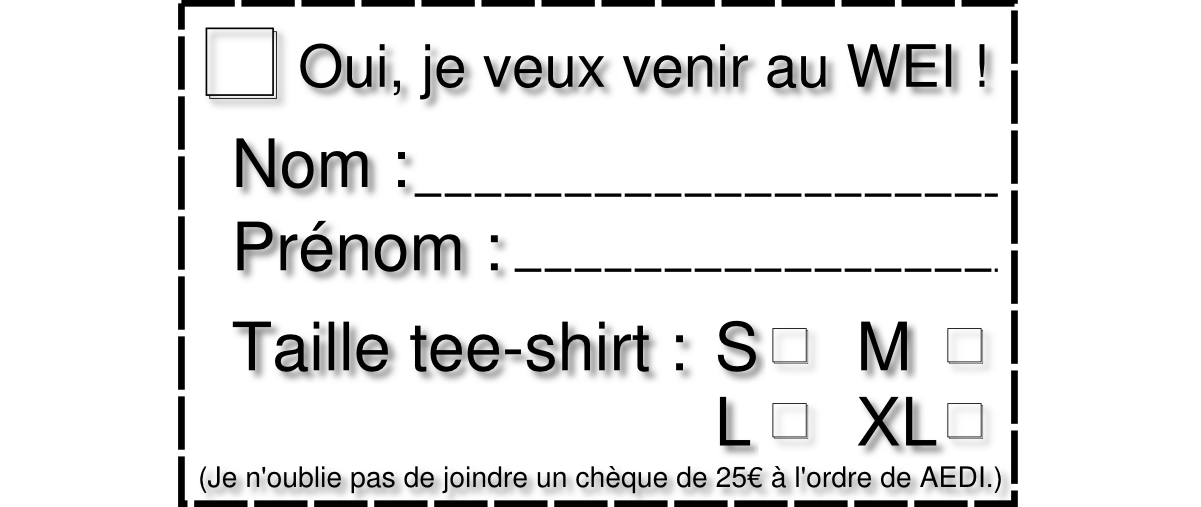
\includegraphics[angle=90, width=6cm]{images/coupon.png}
\end{center}

\newpage
\section{Présentation des orgas}
\orga{images/orgas/armand.jpg}
\paragraph{Armand :} Grand aigri de la troupe, il s'occupera de la sécurité au WEI ! Autant dire que c'est mal barré... Attention pas de blague avec lui ou vous en subirez les conséquences (parole d'ex co-TP !)

\orga{images/orgas/billy.jpg}
\paragraph{Billy :} Le secrétaire de la GPL, infiltré dans l'équipe d'inté pour distiller des propos subversifs à propos de gnous et de manchots.

\orga{images/orgas/clement.jpg}
\paragraph{Clément :} Né avec un appareil photo dans la main, c'est le photographe officiel du départ', vous ne verrez jamais ses yeux qu'à travers un objectif
\columnbreak
~\\
\vspace{0.5cm}

\orga{images/orgas/gael.jpg}
\paragraph{Gaël :} Actuel président de l'AEDI, c'est grâce à lui que le bureau tourne, mais il a néanmoins son petit péché mignon... Si vos petites sœurs sont mineures, ne les ramenez jamais avec vous, vous êtes prévenus.

\orga{images/orgas/guillaume.jpg}
\paragraph{Guillaume} Ancien prépa, il a enfilé ses bas résilles et son tailleur en prenant le poste de secrétaire de l'AEDI. Si vous ne devez retenir qu'une seule chose a propos de lui, c'est deux bras.

\orga{images/orgas/julian.jpg}
\paragraph{Julian :} C'est le maître des jeux, il possède les dés, il a le pouvoir, et vous serez sous son contrôle tôt ou tard...
\clearpage
\orga{images/orgas/julien.jpg}
\paragraph{Julien :}  Le seul, l'unique... Le Resp' Inté ! Grand, beau, fort, musclé, intelligent, menaçant, c'est LUI le maître, il a le précieux !
\orga{images/orgas/loic.jpg}
\paragraph{Loic :} Ancien prépa et glandeur né (ses co-TP témoigneront). Bonjourlesifs dit qu'il possède la plus grosse de tout IF mais c'est uniquement pour pas qu'on le perde lorsque les herbes sont trop hautes.
\orga{images/orgas/marc.jpg}
\paragraph{Marc :} Véritable dictionnaire à acronymes. C'est la seule personne parmi les orgas à pouvoir comprendre le sens réel et profond de cette phrase : «~\texttt{OMG LOL WTF STFU U SUXX L2P U NAAB GTFO !!!1}~»
\orga{images/orgas/nicolas.jpg}
\paragraph{Nical :} Graphiste officiel de l'inté, ses dessins vous feront rêver à d'autres lieux tandis que lui restera enchaîné à notre dominatrice Resp' semaine d'inté.
\orga{images/orgas/paul.jpg}
\paragraph{Paul :} Musicien libriste buvant du café à longueur de journée. Il trouve également le temps d'être le président de la GPL grâce à un secret que j'ose à peine vous dévoiler... C'est une loutre !
\orga{images/orgas/quentin.jpg}
\paragraph{Quentin :} Président du vice de l'AEDI... Vice président pardon. Peu de personnes ont essayé de le suivre côté alcool, et les pauvres ayant tenté l'expérience n'en sont pas ressortis indemnes.
\orga{images/orgas/sandra.jpg}
\paragraph{Sandra :} Responsable de la semaine d'inté, elle dirige ses fidèles escla... serva... compagnons avec toute la grâce qui lui est due.
\vspace{0.5cm}
\orga{images/orgas/sebastien.jpg}
\paragraph{Seb :} L'espion mi-orga mi-bizuth, plus fort que James Bond, il peut utiliser ses nombreux atouts pour se sortir de n'importe quelle situation... Sauf contre Chuck Norris.
\vfill
\columnbreak
\orga{images/orgas/vincent.jpg}
\paragraph{Vincent :} Barman de conviction, il vous fera goûter à de délicieux cocktails. Surnommé Papy Bouli, autant par sa vitesse de déplacement que par son air ronchon, vous le reconnaîtrez à ses «~Oh Marseille !~»
\orga{images/orgas/zaza.jpg}
\paragraph{Zaza :} Trésorière de l'AEDI, elle attend les soldes impatiemment avec son nouveau chéquier ! Responsable WEI, elle dirige le sexe fort d'une main de maître(sse).

\end{multicols}
\begin{center}
    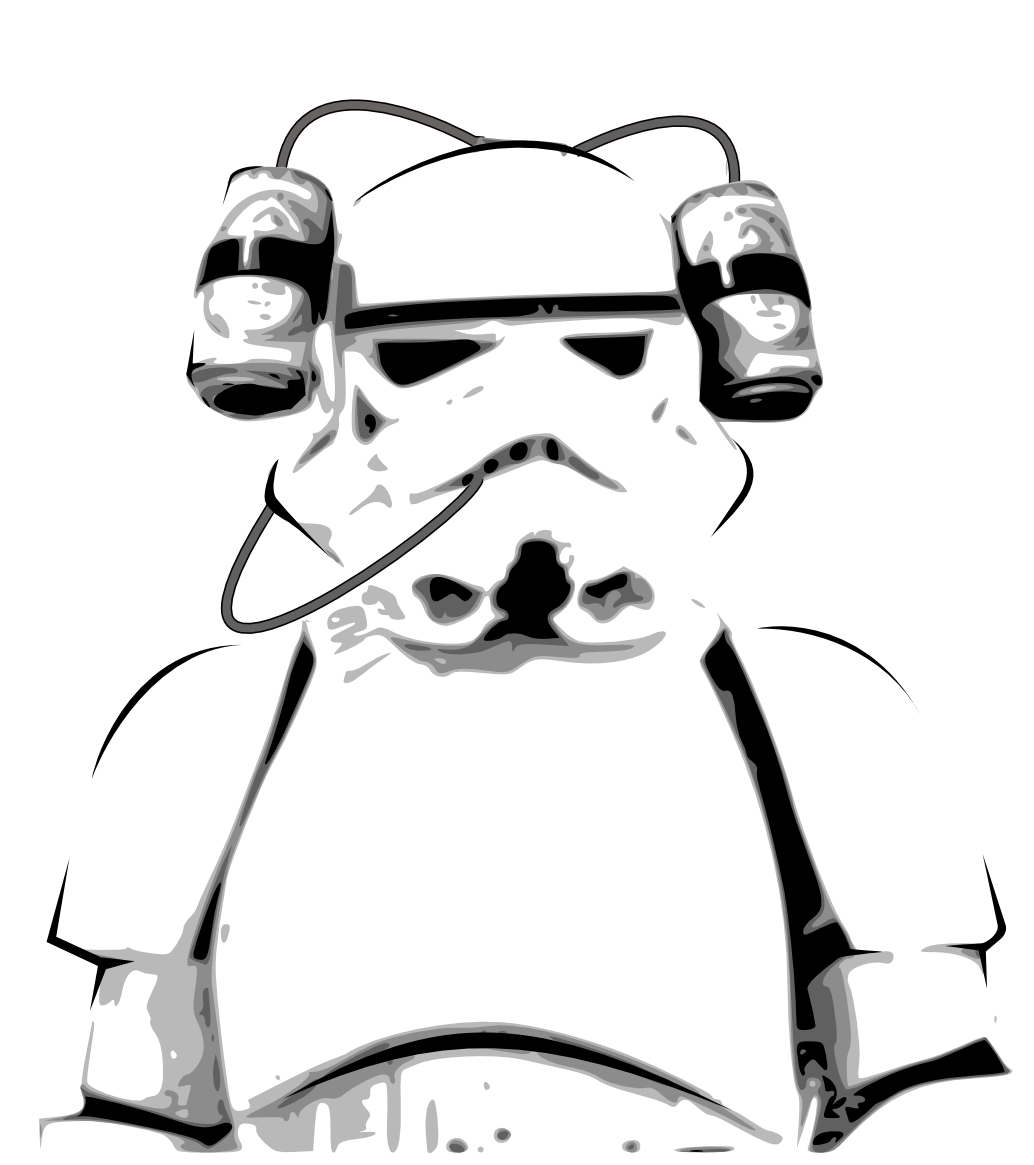
\includegraphics[height=8cm]{images/stormtrooper_biere.png}
\end{center}
\newpage
\begin{multicols}{2}

\newpage
\section{Questionnaire}
\subsection*{Présentation}
\begin{description}
    \item[Nom - Prénom :]
    \item[Surnom]
    \item[Âge :]
    \item[Région d'origine :]
    \item[Sexe :]
    \item[Célibataire~?]
    \item[IF, premier choix ou pas trop ?]
    \item[Des problèmes de santé particuliers ?] (Pour organiser au mieux la
	    semaine).
\end{description}
\subsection*{Photo}
Colle nous donc une jolie photo de toi. Tout contrevenant s'expose à des
poursuites !
\vspace{3cm}
\orga{images/anonymous.jpg}

\subsection*{Test psychologique}
Élaboré par nos plus grands spécialistes, cette section nous permettra d'en
savoir un peu plus sur toi.

\begin{itemize}
    \item \textbf{Donne une description précise du rituel  
	 de l'huitre et du pingouin :}
    \vspace{1cm}

    \item \textbf{Que serais tu si tu étais :}
    \begin{description}
	\item[Chuck Norris:]
	\item[Une série:]
	\item[Un droïd:]
	\item[Un truc vert:]
	\item[Une chanson:]
	\item[Un film:]
	\item[Une heure de la journée:]
    \end{description}
    \item \textbf{Lequel des orgas te parait le plus sympa ?}
    \vspace{1cm}
    \item \textbf{Un ours des forêts du nord met deux jours pour traverser 500m de forêt, pourquoi ?}
    \vspace{2cm}
    \item \textbf{Que cherches tu en venant en IF ?}
    \vspace{3cm}
    \item \textbf{Dessine nous un avion à réaction robotisé intelligent avec une
    lueur maléfique dans les yeux, et des poils soyeux :}
    \vspace{5cm}
    \item \textbf{Pose nous une question :}
    \vspace{2cm}
\end{itemize}
\subsection*{Test de Geekness}
\begin{itemize}
    \item \textbf{Quelle est la différence entre un geek et un nerd ?}
    \vspace{1cm}
    \item \textbf{Combien de langage de programmation maîtrises-tu ?}
    \vspace{1cm}
    \item \textbf{Explique en 3 points pourquoi les produits Apple ne valent
	pas un clou :}
    \vspace{2cm}
    \item \textbf{Combien d'épisode de série regardes-tu en moyenne chaque
	semaine ?} (parce qu'on est un peu à cours, dans l'équipe)
    \vspace{2cm}
    
    \item \textbf{Tu utilises plutôt quotidiennement :}
    \begin{description}
	\item[$\square$] GNU/Linux.
	\item[$\square$] Microsoft Windows.
	\item[$\square$] Apple MacOS.
	\item[$\square$] BSD -- Solaris -- un Atari -- un Amiga.
	\item[$\square$] Un verre à pintes.
	\item[$\square$] Mais qu'est-ce que je fais là ?!
    \end{description}

    \item \textbf{L'info, pour toi, c'est :}
    \begin{description}
	\item[$\square$] Une passion.
	\item[$\square$] Un moyen de se faire pas mal d'argent.
	\item[$\square$] Un bon moyen de faire du management plus tard.
	\item[$\square$] Ta vie.
	\item[$\square$] Un outil.
	\item[$\square$] Marrant.
	\item[$\square$] 42.
    \end{description}
    \item \textbf{T'as deux heures à tuer, tu fais quoi ?}
    \begin{description}
	\item[$\square$] T'as justement une classe à écrire sur un de tes
	projets.
	\item[$\square$] Tu prends un bon bouquin.
	\item[$\square$] T'appelles un pote et tu vas prendre un café en ville.
	\item[$\square$] Tu joues à un jeu (vidéo, ou pas).
	\item[$\square$] Tu fais du sport.
	\item[$\square$] Tu crées un truc (dessin, musique, cuisine, UML, ...).
    \end{description}

    \item \textbf{Comment s'appelle ceci ?}
    \begin{verbatim}
	#include<stdio.h>
	char*f="char*f=%c%s%c;main()"
	"{printf(f,34,f,34,10);}%c";
	main(){printf(f,34,f,34,10);}
    \end{verbatim}
    \vspace{1cm}
    \item \textbf{Une passion dévorante ?} (sport, musique, dessin, etc.)
    \vspace{2cm}
    \item \textbf{Des projets notables en info ?} (i.e. utilisé par plus de monde que ta
	    grand mère, toi, et le prof qui t'as corrigé...)
    \vspace{2cm}
\end{itemize}
\subsection*{Encore photo}
Colle ici une photo de toi complètement stupide :
\begin{center}

\includegraphics[height=5cm, angle=120]{images/anonymous.jpg}
\end{center}

Les meilleurs photos gagneront un passage sur
\url{http://bonjourlesifs.tumblr.com}.

\subsection*{Presque la fin...}
Marque nous quelque chose. Oui, n'importe quoi. Non, vraiment, tu peux te
lâcher, vas-y. Y'a même de la place pour dessiner, écrire de la musique, cet
espace est à toi !
\vspace{8cm}
\subsection{Mais qu'est-ce que je fais avec toutes ces questions ?}
C'est pas bien compliqué, tu les renvoie avec le coupon réponse pour le WEI et
ton chèque à :
\adresseCoupon



Fais quand même attention, le chèque pour le WEI est à mettre à l'ordre de AEDI, pas de la personne ci-dessus !

\vfill
\columnbreak
~
\vfill
\hspace{-5cm}
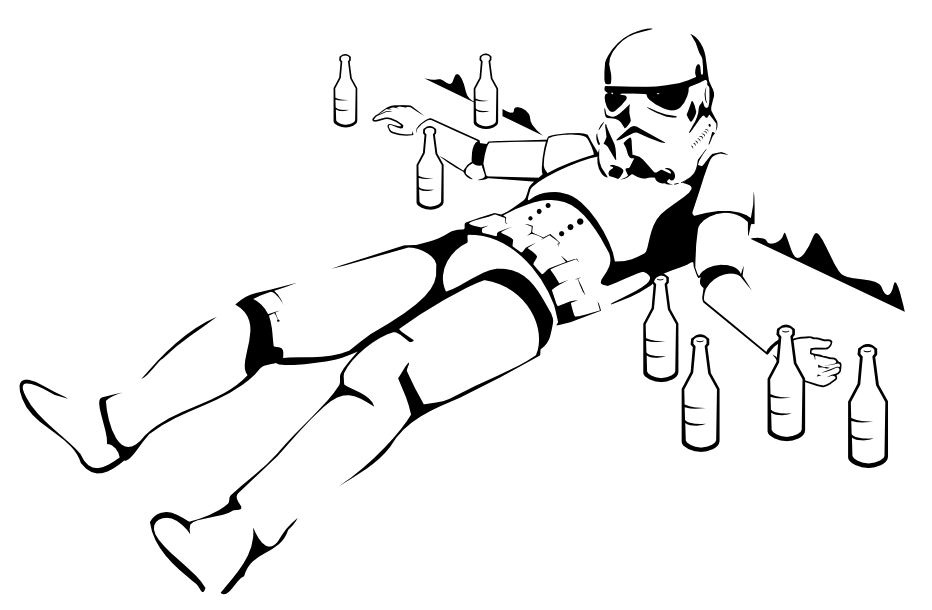
\includegraphics[height=8cm]{images/stormTrooperBourre.png}

\newpage
\section{Présentation pour les admis directs}
    \subsection{L'INSA en gros}
    \vspace{1em}
{
    \footnotesize
    \parindent 0em
    \begin{changemargin}{-1cm}{0cm}
\textbf{M}aintenant que tu as accepté, tu te dis peut-être :\\
\textbf{A}lors, l'INSA c'est quoi au juste ? Ou encore...\\
\textbf{Y} aura-t-il ce que je cherche ?\\

\textbf{T}rès bien, voici le moment où tout ceci te sera dévoilé ! (ou pas)\\
\textbf{H}istoriquement, l'INSA a été fondé en 1957... Comment ? Inintéressant ?\\
\textbf{E}t alors ? Un peu d'histoire ça ne fait pas de mal !\\

\textbf{F}ort heureusement (pour toi), on peut raccourcir un peu tout ça.\\
\textbf{O}sons donc passer sous silence l'historique Insalien...\\
\textbf{R}elativement vite, tu t'habitueras au campus de la DOUA\\
\textbf{C}'est là que tu vivras pour la majorité, entouré d'autres étudiant(e)s\\
\textbf{E}videmment me diras-tu...\\

\textbf{B}on, on va peut-être pouvoir commencer, tu ne crois pas ?\\
\textbf{E}t bien ?\\

\textbf{I}nitialement, ça n'était pas une introduction, mais bon...\\
\textbf{F}inalement, ça l'est.\\
\end{changemargin}
} % End parindent

Bon allez, reprenons.

\vspace{1em}

L'Institut National des Sciences Appliquées est né en 1957, de par la volonté de
former des ingénieurs en grand nombre. L'établissement lyonnais fut bientôt 
rejoint par 4 autres, situés à Toulouse, Rennes, Rouen
et Strasbourg (et oui, il n'y en a pas à Paris !).

\vspace{1em}

L'INSA de Lyon, situé à Villeurbanne (\emph{cherchez l'erreur}) admet en son sein plus
de 5000 étudiants et doctorants, et forme des ingénieurs dans 12 domaines de
spécialisation, couvrant toutes les sciences de l'ingénieur (mécanique,
énergétique, chimie, etc.).

\vspace{1em}

Les nombreuses associations Insaliennes font du campus un lieu à la vie
étudiante dynamique et passionnante. Les divers départements constituant
ce fabuleux ensemble se situent sur le domaine scientifique de la DOUA (100 
hectares, et rien de moins que 26000 personnes sur le site).

    \subsection{INSA, c'est pas que IF}
    Le département IF, c'est 120 élèves par promo, certes, mais les autres départements dans tout ça ?
Car oui, il y a 11 autres départements à l'INSA, pour un total de 800 étudiants par promo.
Peut-être te dis-tu que "Ce ne sont pas des IFs donc on ne les vera jamais !"
Et bien détrompe-toi, tu pourras les rencontrer dans les résidences, les restos,
les associations, les chouilles (\emph{surtout pendant les chouilles...}), mais
aussi les... cours de sport inter-départ' ou encore les cours de langues
étrangères! (\emph{oui c'est important de préciser étrangères pour éviter les
ambiguïtés...}) Vous serez alors dans une atmosphère conviviale pour
retrouver les joies de votre LV2 favorites.

Outre ces autres départements, il y a aussi les fameux PC ou encore Premier
Cycle qui correspondent à la prépa intégrée INSA et qui consiste à préparer les
étudiants à entrer dans les différents départements que compte l'INSA à travers
toute la France ! Pendant ces deux ans, ils n'ont pas étudié exactement les
mêmes disciplines qu'un élève de prépa en lycée aura pu étudié. Ils font bien
évidemment des maths, de la physique, et toutes ces matières que les BTS/DUT
adorent, mais également du dessin industriel ou encore de la programmation en
PASCAL... (\emph{yeah c'est la fête !}).


Ainsi, ne soyez pas étonnés de voir que certains IFs connaîtront déjà des
personnes de ces départements, car oui, une grande proportion a fait le Premier
Cycle (environ 85 \%). Mais rassurez-vous, ils sont tellement nombreux  (plus de
800 par promo) qu'ils ne se connaissent pas tous et par conséquent, vous
ne serez pas confrontés à un groupe soudé dès le départ. Ainsi, pas de souci
pour s'intégrer parmi eux. Et puis pour tout vous dire, ils sont plutôt
accueillant, parole d'admis direct.

Une dernière petite chose à noter : il y a des filières internationales à
l'INSA, et ces dernières accueillent une grande proportion d'étudiants étrangers
et.... une bonne partie viennent en IF! Idéal pour se familiariser avec d'autres
cultures! Voici les nationalités que vous pourrez rencontrer par exemple:
Chinoise, Roumaine, Italienne, Brésilienne, Mexicaine, Slovaque, Bretonne,
Tunisienne... Il y a aussi quelques français parmi tout ça.

    \subsection{Campus}
    Le campus ? Rien de moins que 100 hectares... Et tu n'en verras probablement pas
la moitié !

\vspace{1em}

Le campus est une véritable ville à l'intérieur de Villeurbanne, de la taille
d'un arrondissement Lyonnais en superficie et d'une petite ville
démographiquement parlant ! Tu pourras y trouver tout ce dont tu as besoin pour vivre !
Un stock de jeunes filles assez limité (le stock, pas les filles) ou un stock de jeunes hommes illimité, mais
aussi des laveries se trouvant dans les résidences pour toujours être au top de
la classe avec ton t-shirt de panda roux, un bar associatif répondant au doux nom de «~K-fêt~»
pour se jeter un verre vraiment pas cher après un TP prise de tête, en écoutant
la bonne vieille fanfare, la Coop (l'épicerie du BdE) pour des petites courses
(\emph{les coursinettes ?}) à un tarif assez avantageux, et bien d'autres choses encore !

\vspace{1em}

J'allais oublier ! Depuis ta chambre, tu sors la tête par la fenêtre et même pas
besoin de téléphone, tu peux dialoguer en live avec des centaines de nanas et
de gars près de chez toi (\emph{enfin surtout des gars}) ! Finis les SMS surtaxés et
les notes salées !

\vspace{1em}

Alors pourquoi sortir du campus te demandes-tu ? Mais pourquoi donc se risquer
dans la «~grande~» ville de Lyon alors que tu n'es qu'un pauvre geek apeuré et effrayé par la
société contemporaine ? Parce que c'est Lyon ? Que c'est une superbe ville ?
Parce que la fac de lettres, accessoirement le repère de toutes les nanas, se
situe au coeur de Lyon ? Parce que pour «~shaker son booty~» ~(comme ils disent dans
les clips de rap US) il faut bouger sur la presqu'île ? Pour avoir la réponse à
ces questions, il te faudra être patient et attendre la partie du poly dédiée à la ville
de Lyon et rédigée par un non-lyonnais qui vient de la cambrousse mais
qui connaît quand même assez la ville pour en parler !

\vspace{1em}

D'ailleurs petite précision, dans ta promo à l'INSA de Lyon, tu ne trouveras
que peu de Lyonnais... Alors, heureux ?

    \subsection{Associatif}
    Tu cherches une association particulière ? Alors tu devrais pouvoir la trouver ici !
Plus d'une centaine d'associations se partagent la vedette sur l'INSA, du club photo au club mangas, en
passant par les clubs danse, voile (pour ceux
voulant faire le tour de France à la voile), magie, ou encore ceux
préparant les grands évènements ayant lieu sur le campus, tout y est, il ne
reste plus qu'à réussir à se décider ! Et le choix sera dur...
N'hésite pas, associe-toi à ces valeureux groupes faisant vivre le campus ! (\emph{et accessoirement, gagne un niveau en «~je fais autre chose que
des TP~» !})

\vspace{1em}

Voilà un léger (mais alors infiniment léger) descriptif des assos :

\paragraph{Arts et Spectacles}
Le ciné-club propose des projections de films à prix... minime ?
Des associations musicales et théâtrales n'attendent que toi pour casser les planches et organiser encore plus de merveilleux spectacles.

\paragraph{Culture et Loisirs}
La danse, la lecture, l'astronomie, la musique ou l'électronique t'intéressent ?
Alors ne t'en fais pas, il y a obligatoirement une asso pour toi !
Tu es reporter dans l'âme ? Alors rejoins les rangs de l'Insatiable, le journal gratuit des étudiants, publié penta-annuellement !

\paragraph{Humanitaire et Social}
Bien qu'ingénieur, nous restons humains ! (\emph{ou orangs-outans...})
Le Karnaval Humanitaire organise ainsi chaque année une semaine de festivités,
sous un chapiteau installé sur le campus, afin de financer des projets
humanitaires.
Handizgoud a pour objectif de sensibiliser les futurs cadres à l'insertion
professionnelle des personnes handicapées.

\paragraph{Sports}
Que tu sois débutant ou champion, que tu veuilles faire de l'aviron, du
basket, du rugby, du volley, des combats de robots (\emph{euh non, ça
c'est en IF, et en plus c'est vrai...}), tu pourras trouver tout ce que tu veux !

\vspace{1em}

Pour ceux avides de détails sur les associations, je vous conseille le site 
\url{http://bde.asso.insa-lyon.fr/botinsa/} qui vous fournira toutes les
informations voulues.


    \subsection{BdE}
    Le BdE est l'entité qui chapeaute tout l'associatif Insalien. Ayant élu résidence à
la MdE (maison des étudiants, bâtiment Le~Thélème), il organise notamment le
Gala, l'intégration des premières années, peut te dépanner avec la COOP, l'épicerie
étudiante, publie le Bot'INSA, l'annuaire des assos de l'INSA, ainsi que l'agenda.
Il gère aussi les laveries, les photocopieurs, il est possible d'y acheter des
tickets de tram, des timbres, et on peut y louer des amphis, des salles de soirée,
des appareils à crêpes, à raclette...
Bref, le BdE est absolument indispensable à la vie à l'INSA~!


    \subsection{Gros évènements}
    De nombreux évènements sont organisés toute l'année sur le campus, cette section
vise à en présenter quelques-uns.

\paragraph{Le Gala}
Il se tient à la mi-février, à l'occasion de la remise des
diplômes de nos chers grands parrains et grandes marraines. Aux réjouissances :
des jeux, des spectacles, du champagne, et ce dans un univers différent chaque année !
Pas question donc de te ramener dans ton vieux jean délavé (mais confortable) ce
jour-là : tenue de soirée exigée. Sors donc ton plus beau costard, dévalise
l'ensemble des boutiques de Lyon pour trouver la robe de tes rêves, mais fais un
effort. Le Gala, c'est THE évènement classy de l'année.

\paragraph{Le Karnaval Humanitaire}
Grandes soirées en perspective, avec animations, concerts (dans les mouvances
reggae, electro et dub), défilé de chars. Un grand chapiteau est même monté sur le
campus, devant la pelouse des Humas. L'idée de la manifestation est de
récolter des dons afin de réaliser de nombreuses actions humanitaires.


 \paragraph{Les 24h de l'INSA}
 L'histoire veut que cet évènement soit dédié à deux étudiants qui, un
 week-end ou ils n'avaient plus de connection internet, se sont mit à courir
 autour de l'INSA, et ce pendant 24h. Depuis, chaque année, des dizaines de
 personnes viennent faire de même, que ce soit à vélo, en roller, à la nage ou à
 pied, et de nombreuses courses prennent part tout au long des deux jours. Pour les
 moins sportif, des concerts et de nombreuses animations ont lieu sur le
 campus. Crois-moi, tu ne vas pas t'ennuyer pendant les 24h !


    \subsection{Lyon en gros}
    Être étudiant à l'INSA, c'est également être étudiant à Lyon et de ce fait, ça
catapulte du pâté issu de l'agriculture biologique (c'est bien quoi) !

Bienvenue dans la troisième plus grosse ville de France, une ville
qui bouge énormément, surtout quand comme beaucoup (par exemple l'auteur de ce
paragraphe) tu es issu(e) d'une petite bourgade de 50 habitants et 150 moutons.

Lyon c'est 450000 habitants, 9 arrondissements placés un peu aléatoirement sur
la carte, 2 fleuves, 4 lignes de métro, 4 lignes de tram, une centaine de lignes
de bus régulières et des évènements tout au long de l'année ! Mais c'est aussi 3
universités nommées respectivement Lyon 1 - Université Claude Bernard (c'est
nous ça !), Lyon 2 - Université Lumière et Lyon 3 - Université Jean
Moulin, totalisant près de 125000 étudiants !

Lyon est considérée comme l'embouchure de la vallée du Rhône, ce qui lui confère
une situation géographique extrêmement intéressante ! En TGV, tu es
à 2h de Paris et de Marseille ! Mais tu es également à 1h30 des pistes de ski,
de quoi passer des week-end de détente parfaits entre amis, ou bien choisir de
pratiquer le ski comme activité physique en sport ! (attention, les places sont limitées, alors soyez réactifs)

Ce qui est dingue, c'est qu'avec tout ça, cette ville a l'avantage de conserver
des loyers relativement peu élevés comparés à d'autres grandes villes ! Un bon point pour nous, les étudiants.

Tout d'abord, il te faudra quelque chose d'essentiel pour apprendre à découvrir
Lyon. Ce quelque chose s'intitule «~Le Petit Paumé~», un bouquin façon guide
Michelin qui te renseignera sur l'ensemble des adresses incontournables de ta
nouvelle ville ! Ce guide est gratuit, et est distribué en octobre ou novembre
selon les années dans les endroits stratégiques de Lyon. Notons les
principaux : sur le campus, devant le restaurant Castor \& Polux (le \emph{Beurk} pour les
intimes), au BdE, ou encore Place Bellecour. Profitez-en, c'est gratuit
et c'est rédigé par des étudiants comme vous !

Justement, rentrons un peu plus dans les détails et voyons ce qu'il est
intéressant de savoir à Lyon. Tout d'abord, la ville est construite à la
confluence de deux fleuves, le Rhône et la Saône, donnant naissance à ce que
l'on appelle la «~presqu'île~», correspondant aux premier et deuxième arrondissements.
C'est sur cette presqu'île qu'est concentrée l'essentiel de l'activité festive
de la ville. Envie d'aller boire un verre ? Tu auras le choix parmi des
centaines de bars ! Un petit creux ? Des restaurants à profusions et notamment
les fameux bouchons Lyonnais afin de manger généreusement des spécialités de
Rhône-Alpes (et pas que) pour 10€ ! C'est le cœur de la ville !

Lyon c'est également des coins insolites à découvrir, et une ville extrêmement
touristique. Comment citer Lyon sans parler de la basilique de Fourvière,
surplombant la ville au sommet de la colline de... Fourvière ? Comment citer
Lyon en oubliant de parler de la fameuse Place Bellecour et de la statue de
Louis XIV ? Comment citer Lyon sans parler de la fontaine de Bartholdi (artiste
ayant réalisé la statue de la liberté pour les incultes) située
Place des Terreaux ?

Lyon est une ville très riche historiquement parlant ! Vous pourrez découvrir le
vieux Lyon et ses bâtisses moyenâgeuses en mangeant une glace artisanale. Vous
aurez l'occasion parcourir les nombreuses traboules, petits chemins étroits, passant dans
des lieux étranges de la ville. Vous
pourrez également contempler de magnifiques trompe l'œil à la Croix Rousse, une
autre colline surplombant la ville, avec notamment la fameuse maison des Canus.


Vous pourrez redécouvrir la ville le soir en vous
baladant sur les bords de la Saône ou lors de la fête des Lumières début décembre,
lorsqu'elle revêt son plus bel apparat pour charmer les touristes
venus du monde entier pour admirer cette mise en scène spectaculaire !
Vous aurez l'opportunité de participer à des centaines de festivals culturels gratuits
! Vous pourrez sortir en boîte sur les péniches, vous remplir les
oreilles de Jazz jusqu'à 5h du matin ou bien faire des barbecues
jusqu'à pas d'heure au parc de Parilly. Vous pourrez essayer de
charmer de jeunes demoiselles, le soir, sur la place Bellevue sur les
pentes de la Croix Rousse. Vous pourrez visiter des vestiges gallo-romains
à Fourvière. Vous pourrez même voir le plus célèbre octogénaire
Lyonnais, Jean-Pierre, courir sur les berges du Rhône tous les soirs et
l'encourager comme le font les centaines d'étudiants venant passer leur
soirée dans l'herbe ! (pour en savoir plus sur notre ami Jean-Pierre : \url{http://bit.ly/cMbVnA})

Et lorsque vous aurez la chance de connaître les grèves des TCL (exploitant du
réseau de transports en commun) et que vous marcherez la nuit, vous vous
rendrez compte à quel point vous avez de la chance d'être venus à Lyon !


    \subsection{Manuel d'arrivée}
    \subsubsection{Comment venir à l'INSA}
    Deux choix pour arriver sur Lyon :

\vspace{1em}

Débutons par celui posant le plus de problèmes (encore que) : la voiture !
Une fois sur le périphérique lyonnais (oui jusqu'ici, tu dois choisir de tourner à droite ou à gauche en jouant à pile ou face !)
il te faut sortir à la «~\textbf{Porte de la Doua}~» ou «~\textbf{Porte de
    Croix-Luizet}~» (peut-être plus facile d'accès...)
et ensuite, en suivant les panneaux «~Campus scientifique de la DOUA~»
tu tomberas sur l'une des multiples entrées de l'INSA !

\vspace{1em}

L'autre choix, plus écologique : le train !
Si tu arrives à la gare Perrache, deux solutions :
\begin{itemize}
    \item Soit tu prends le \textbf{Métro A} (en rouge sur les plans) afin
    d'aller jusqu'à \textbf{Charpennes - Charles Hernu} pour une
    petite correspondance avec le \textbf{Tramway T1} direction
    \textbf{IUT Feyssine}. Tu sortiras alors à l'arrêt
    \textbf{La Doua - Gaston Berger}, et tu seras arrivé(e) directement sur le campus, au pied de notre cher bâtiment.

    \item Soit tu prends directement le \textbf{Tramway T1}, et tu
    attends l'arrêt \textbf{La Doua - Gaston Berger}. Oui, c'est
    beaucoup plus simple, mais c'est aussi plus long en fonction des
    temps d'attente aux correspondances.
\end{itemize}

\vspace{1em}

Si tu arrives à la gare Part-Dieu, c'est encore plus simple ! Le
\textbf{Tramway T1} s'arrête pour te prendre juste à la sortie de la gare,
coté \textbf{Vivier Merle}, pile devant le centre commercial \textbf{La Part-Dieu}, pour
t'emmener tout de suite à l'INSA (comme précédemment, arrêt \textbf{La Doua - Gaston Berger}).

\vspace{1em}

Que ce soit en voiture ou en train, nous te conseillons d'acheter un carnet de
10 tickets TCL, au modeste prix de 11.90€ pour les étudiants (pour
les trouver aux bornes, il faut chercher quelques secondes !). Ces derniers te
permettront d'utiliser toutes les correspondances des transports TCL (métro,
tram, funiculaire, bus, trolleybus) et ce pour une durée d'une heure par ticket 
(malheureusement, comme tu le verras rapidement, un retour ne peut se faire
avec le même ticket que l'aller... Alors il faut filouter !).


    \subsubsection{On fait quoi une fois arrivé}
    Trouver sa chambre et aller s'inscrire, voilà les deux activités de la journée !

Si tu es chargé(e) comme une mule, la première est prioritaire, il faut donc te
rendre à la \textbf{Direction Des Résidences} (DDR), qui se trouve au pied des résidences
G et J (voir la carte, numéro 6) afin de récupérer ton «~Bon d'emménagement~» (\emph{ainsi que 600 points
d'expérience et un niveau en ~«attente de l'administration~»}).
Tu pourras ensuite aller dans ta résidence afin de récupérer tes
clés et effectuer un état des lieux (en échange du bon).

La seconde activité est un petit parcours du combattant mettant à profit tes 
jambes et ta patience, mais nous ne voulons pas tout dévoiler maintenant et
te laissons découvrir cette partie de franche rigolade (\emph{ou pas}) par toi-même !
(petit conseil : n'oublie pas le stand d'inscription aux restos du campus, ainsi que le
 stand de l'agence comptable, te permettant d'opter pour le prélèvement bancaire
 automatique du loyer de ta chambre si tu le souhaites). Tout ça se passe en 9,
dans le bâtiment Pierre de Fermat, (void la carte, page \pageref{plan}).

Et voilà, fin de la journée... Euh, en fait, non.
Et oui, car vous pourrez alors venir au département où de gentils et merveilleux
orgas (\emph{on pourrait presque dire que ce sont des bisounours tellement ils sont
merveilleux nos orgas !}) t'attendent, toi et tes parents, pour effectuer
la visite du département ! (un petit en-cas avant la grande visite du lendemain) 

    \clearpage
\section{Lexique}
Bon, la première fois qu'on est rentré dans le départ', on a rien compris, d'où
ce petit glossaire, qui ne saurait être exhaustif :

\plex{AEDI}{L'association des élèves du département informatique... C'est elle qui organise les grands évènements de ta scolarité en IF, que ce soit le week-end d'intégration, le week-end ski, les rencontres IF's, les barbecues, le concert IF...}
\plex{Associations}{Composantes essentielles à la vie sur le campus. Attention à l'overdose pour les plus gourmands !}
\plex{C++}{La matière à ne pas négliger, et aussi la plus grosse session rattrapage.}
\plex{Café}{Boisson officielle du département, distribuée en salle détente (sauf en cas de pénurie).}
\plex{Cobinôme}{Partage ton binôme.}
\plex{Copain}{Partage ton pain.}
\plex{Copine}{Stocks limités, prévoir par avance !}
\plex{Co-TP}{Partage "tes P" (et tes galères en salle machine).}
\plex{Fil rouge}{Un projet libre, non noté, qui remplace un TP dans l'année. Il est optionnel, et prend souvent beaucoup plus de temps que le TP qu'il permet de faire sauter.}
\plex{Gaston Berger}{Ton compagnon de réveil pour l'année.}
\plex{GNU/Linux}{Un vrai système d'exploitation. Pour certains.}
\plex{GPL}{La meilleure association de tout l'INSA, de manière complètement objective. Ahem.}
\plex{\url{http://bonjourlesifs.tumblr.com}}{Presque aussi bien que \url{http://bonjourbde.fr}, ce site te délivre une fois par jour une photo de tes futurs parrains.}
\plex{IUT}{Des bon gros codeurs qui ont tendance à pleurer en maths. Chacun son truc. Le départ' en accueille environ une vingtaine par an.}
\plex{Khepera}{Selon les gens, leur meilleur souvenir ou un de leurs pires cauchemars.}
\plex{Loutre}{Le mot «~schtroumpf~» de l'étudiant en informatique !}
\plex{Mac-users}{Seront-ils plus de deux cette année ?}
\plex{Martius}{Un imposteur, on ne sait toujours pas ce qu'il fait là.}
\plex{Micromachine}{Un des TP les plus cools de l'année !}
\plex{Nuit blanche}{Tu verras, on s'y fait.}
\plex{Parrain}{Ton parrain de promo, c'est Altran. Tes parrains de bizutage et d'intégration, c'est nous !}
\plex{RIFs}{Rencontres IFs : mets-toi sur ton 42 et pars à la chasse au stage dans ce forum de recrutement propre au départ' !}
\plex{Salle détente}{Des canapés pour dormir, du café pour vivre et un PC pour mettre de la musique. What else ?}
\plex{SGM}{Les locataires d'en-dessous.}
\plex{The cake}{It's a lie. Definitely.}
\plex{Turne}{Ta chambre, si tu habites sur le campus.}
\plex{Troll}{Attitude volontaire d'un protagoniste d'un débat à lancer stratégiquement une remarque complètement infondée et à fort potentiel polémique, telle que «~Windows, c'est de la merde~». Sport officiel de l'équipe d'inté.}
\plex{Twitter}{Un truc qui sert à rien au début, et dont on a du mal à se passer ensuite.}
\plex{Windows}{Quoiqu'on en dise, au final, ce sera toujours lui le vainqueur.}

\clearpage
\end{multicols}
\section{Plans}\label{plan}
\subsection{Plan du campus}
\begin{minipage}{0.7\textwidth}
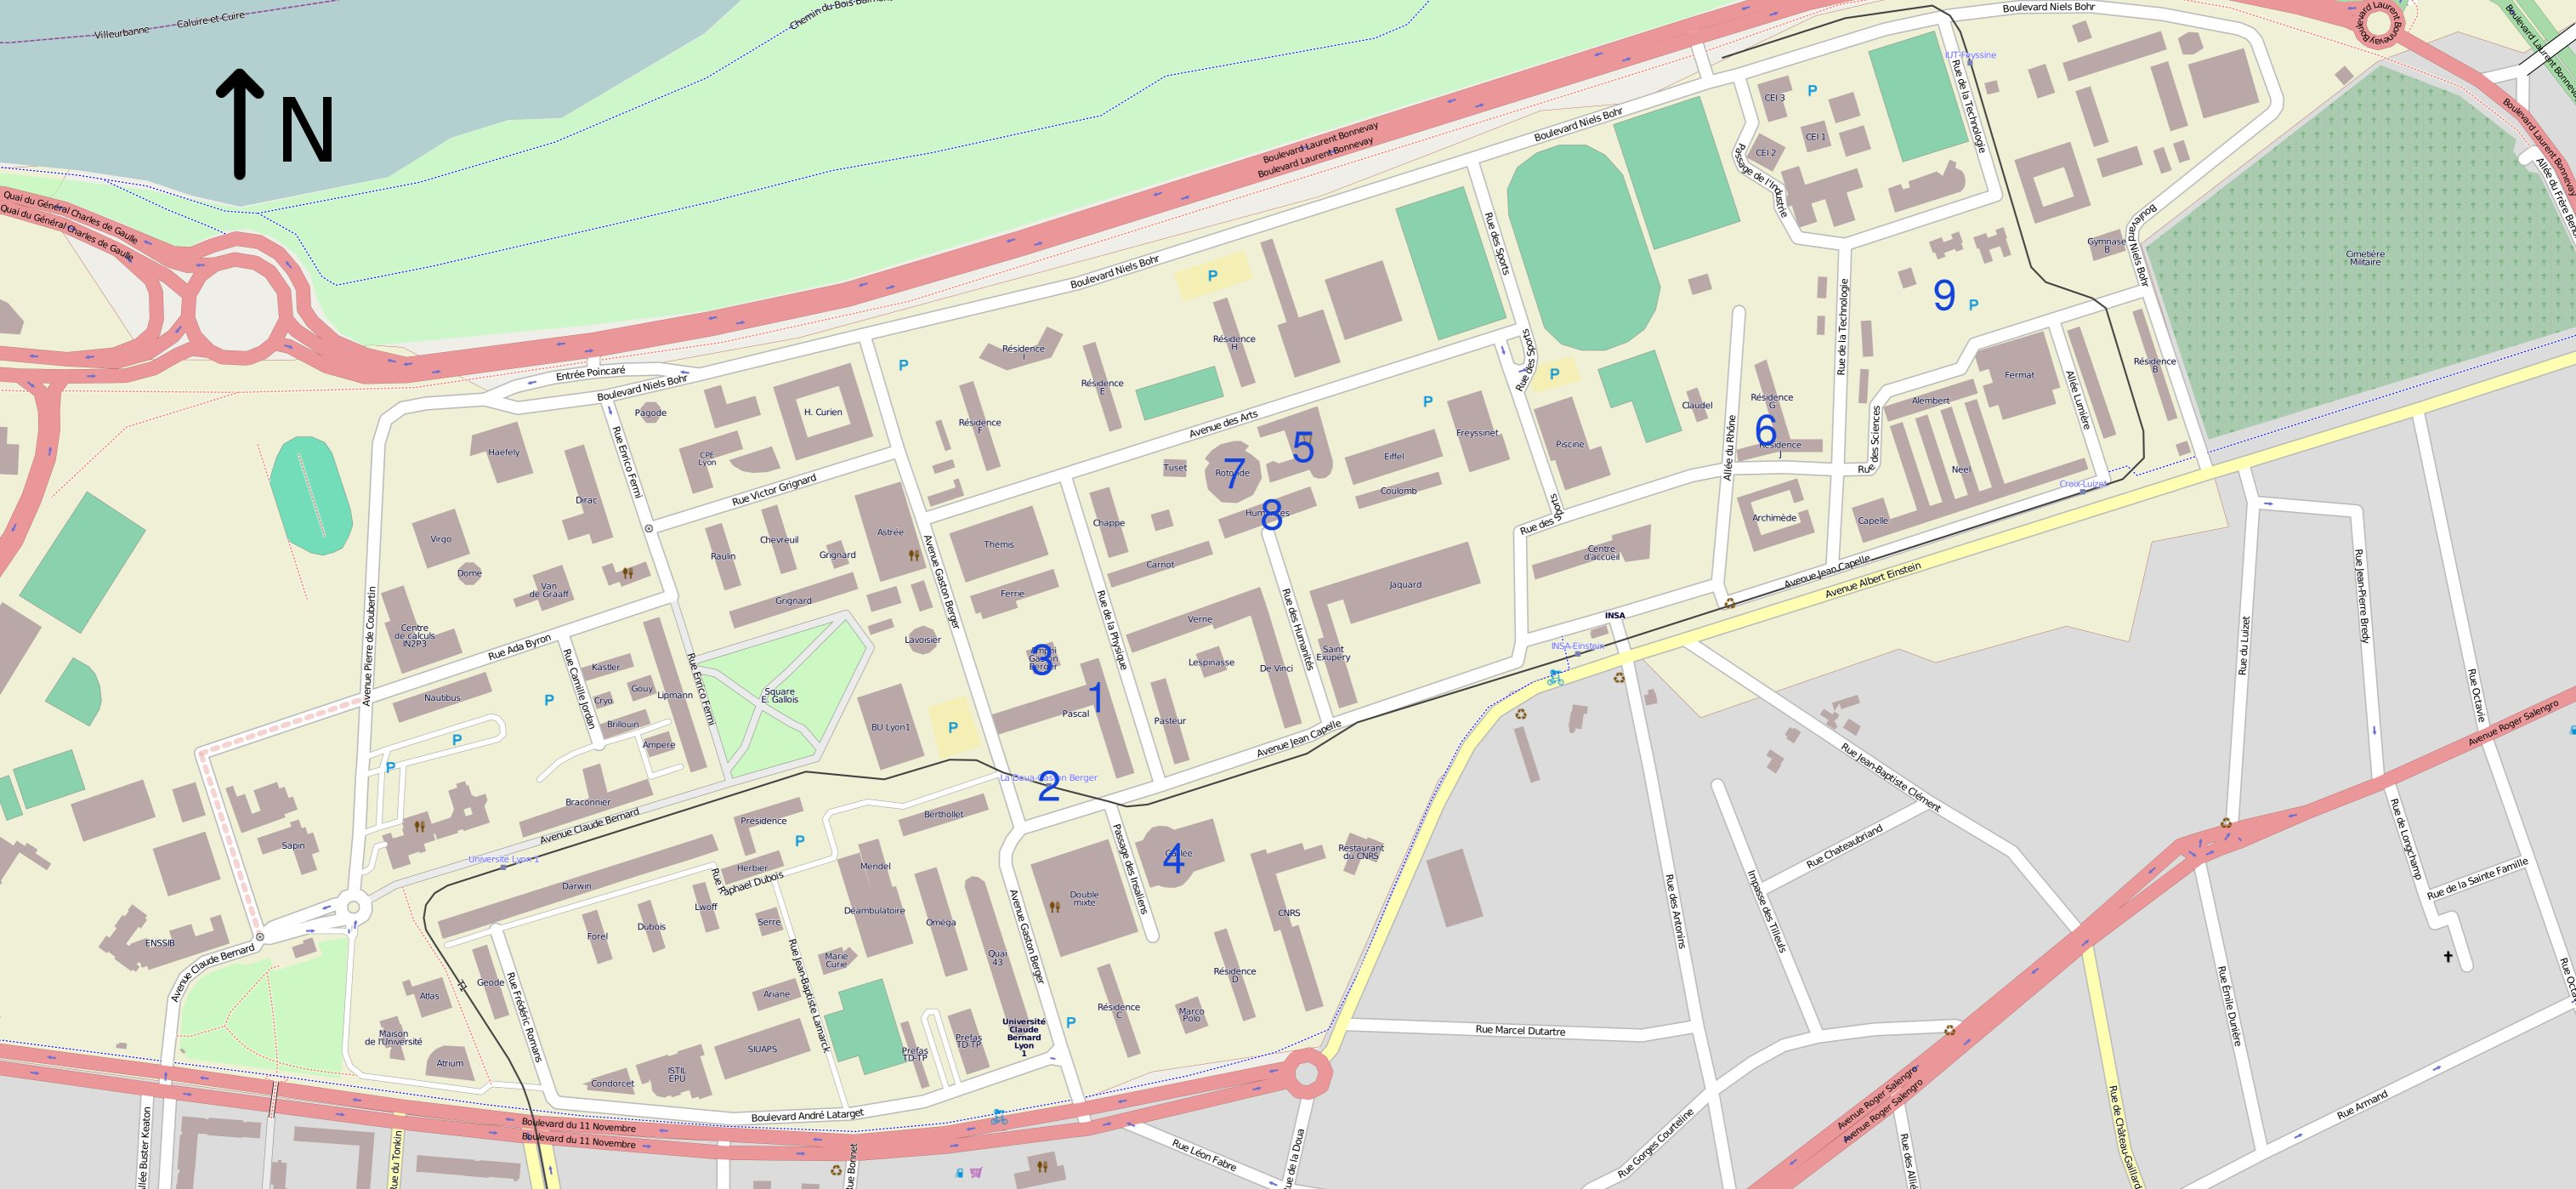
\includegraphics[width=24cm, angle=90]{images/planDoua.jpg}
\end{minipage}
\begin{minipage}{0.3\textwidth}
\textbf{Légende}
    \begin{enumerate}
	\item Département
	\item Amphi
	\item Arrêt de tram
	\item Restaurants
	\item MdE, K-Fêt
	\item Direction des résidences
	\item Rotonde
	\item Bâtiment des Humanités
	\item Bâtiment Pierre de Fermat
    \end{enumerate}
   \vspace{2cm} 
    Il est possible de zoomer sur l'image pour avoir le nom des résidences et
    des bâtiments de manière plus lisible.
\end{minipage}
\newpage

\subsection{Plan TCL}
\hspace{-2cm}
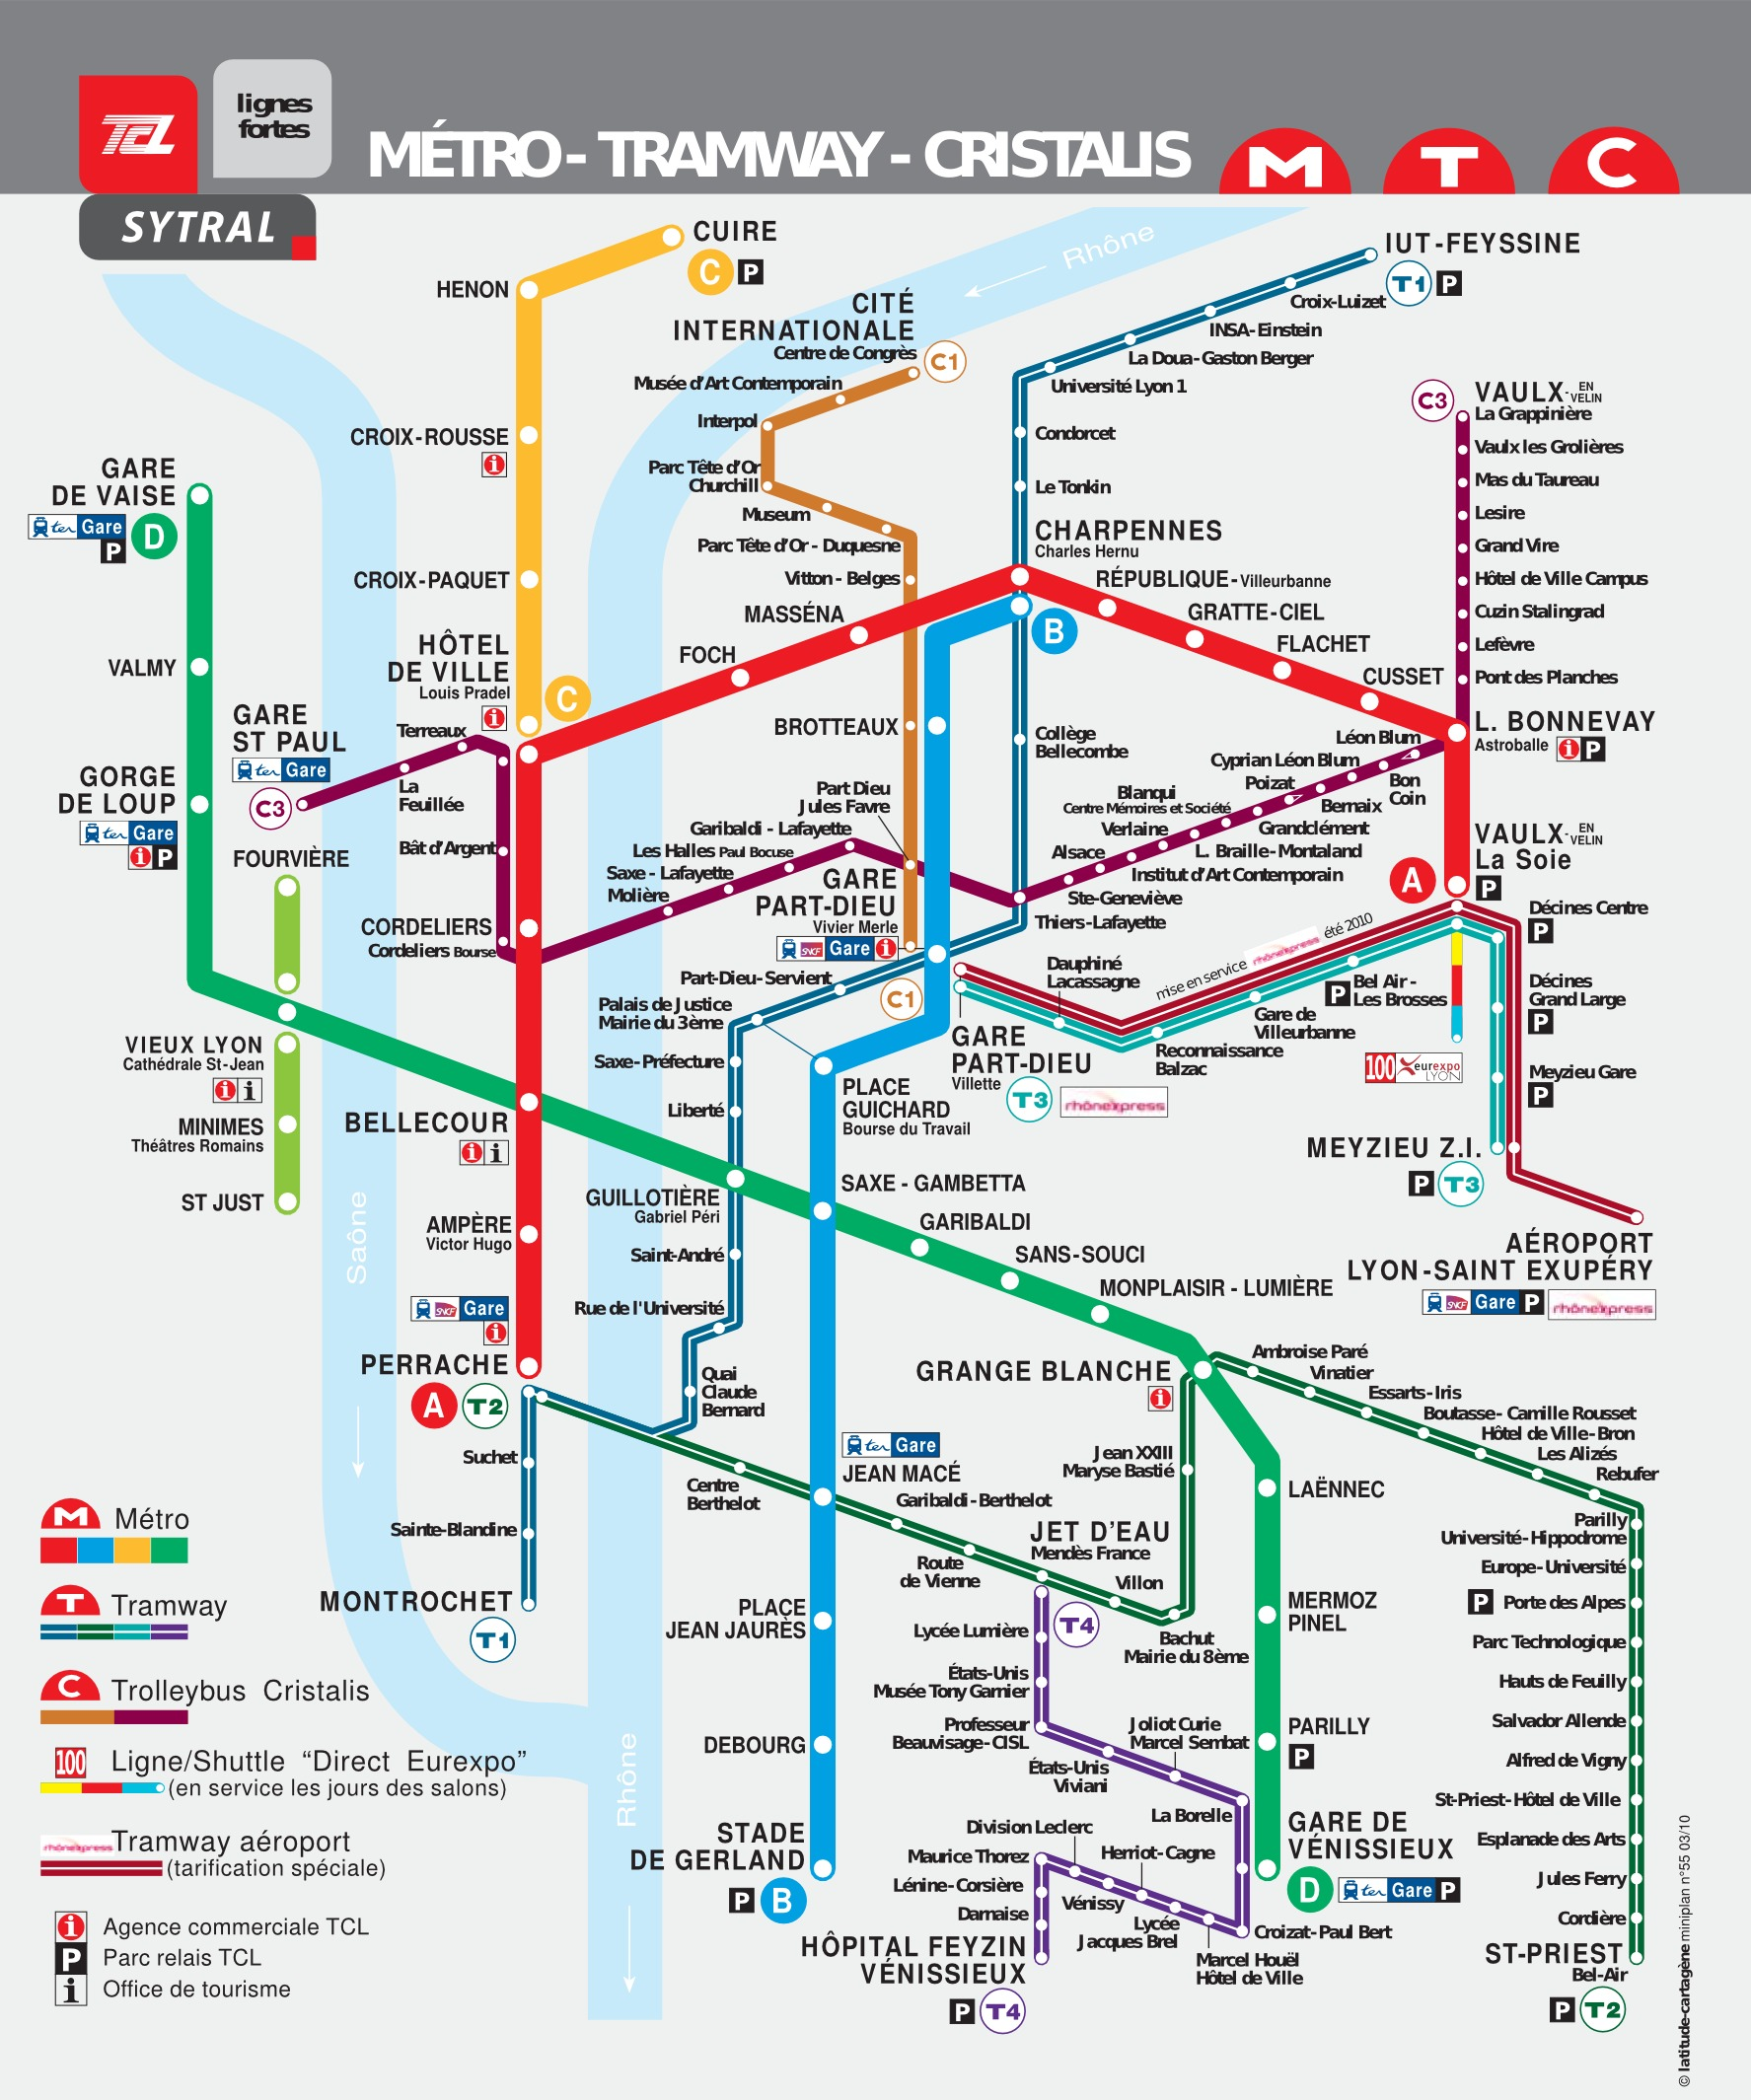
\includegraphics[width=19cm]{images/planTCLFullRes.jpg}

\newpage 
\subsection{Plan du départ (2\up{e} étage)}
\begin{center}
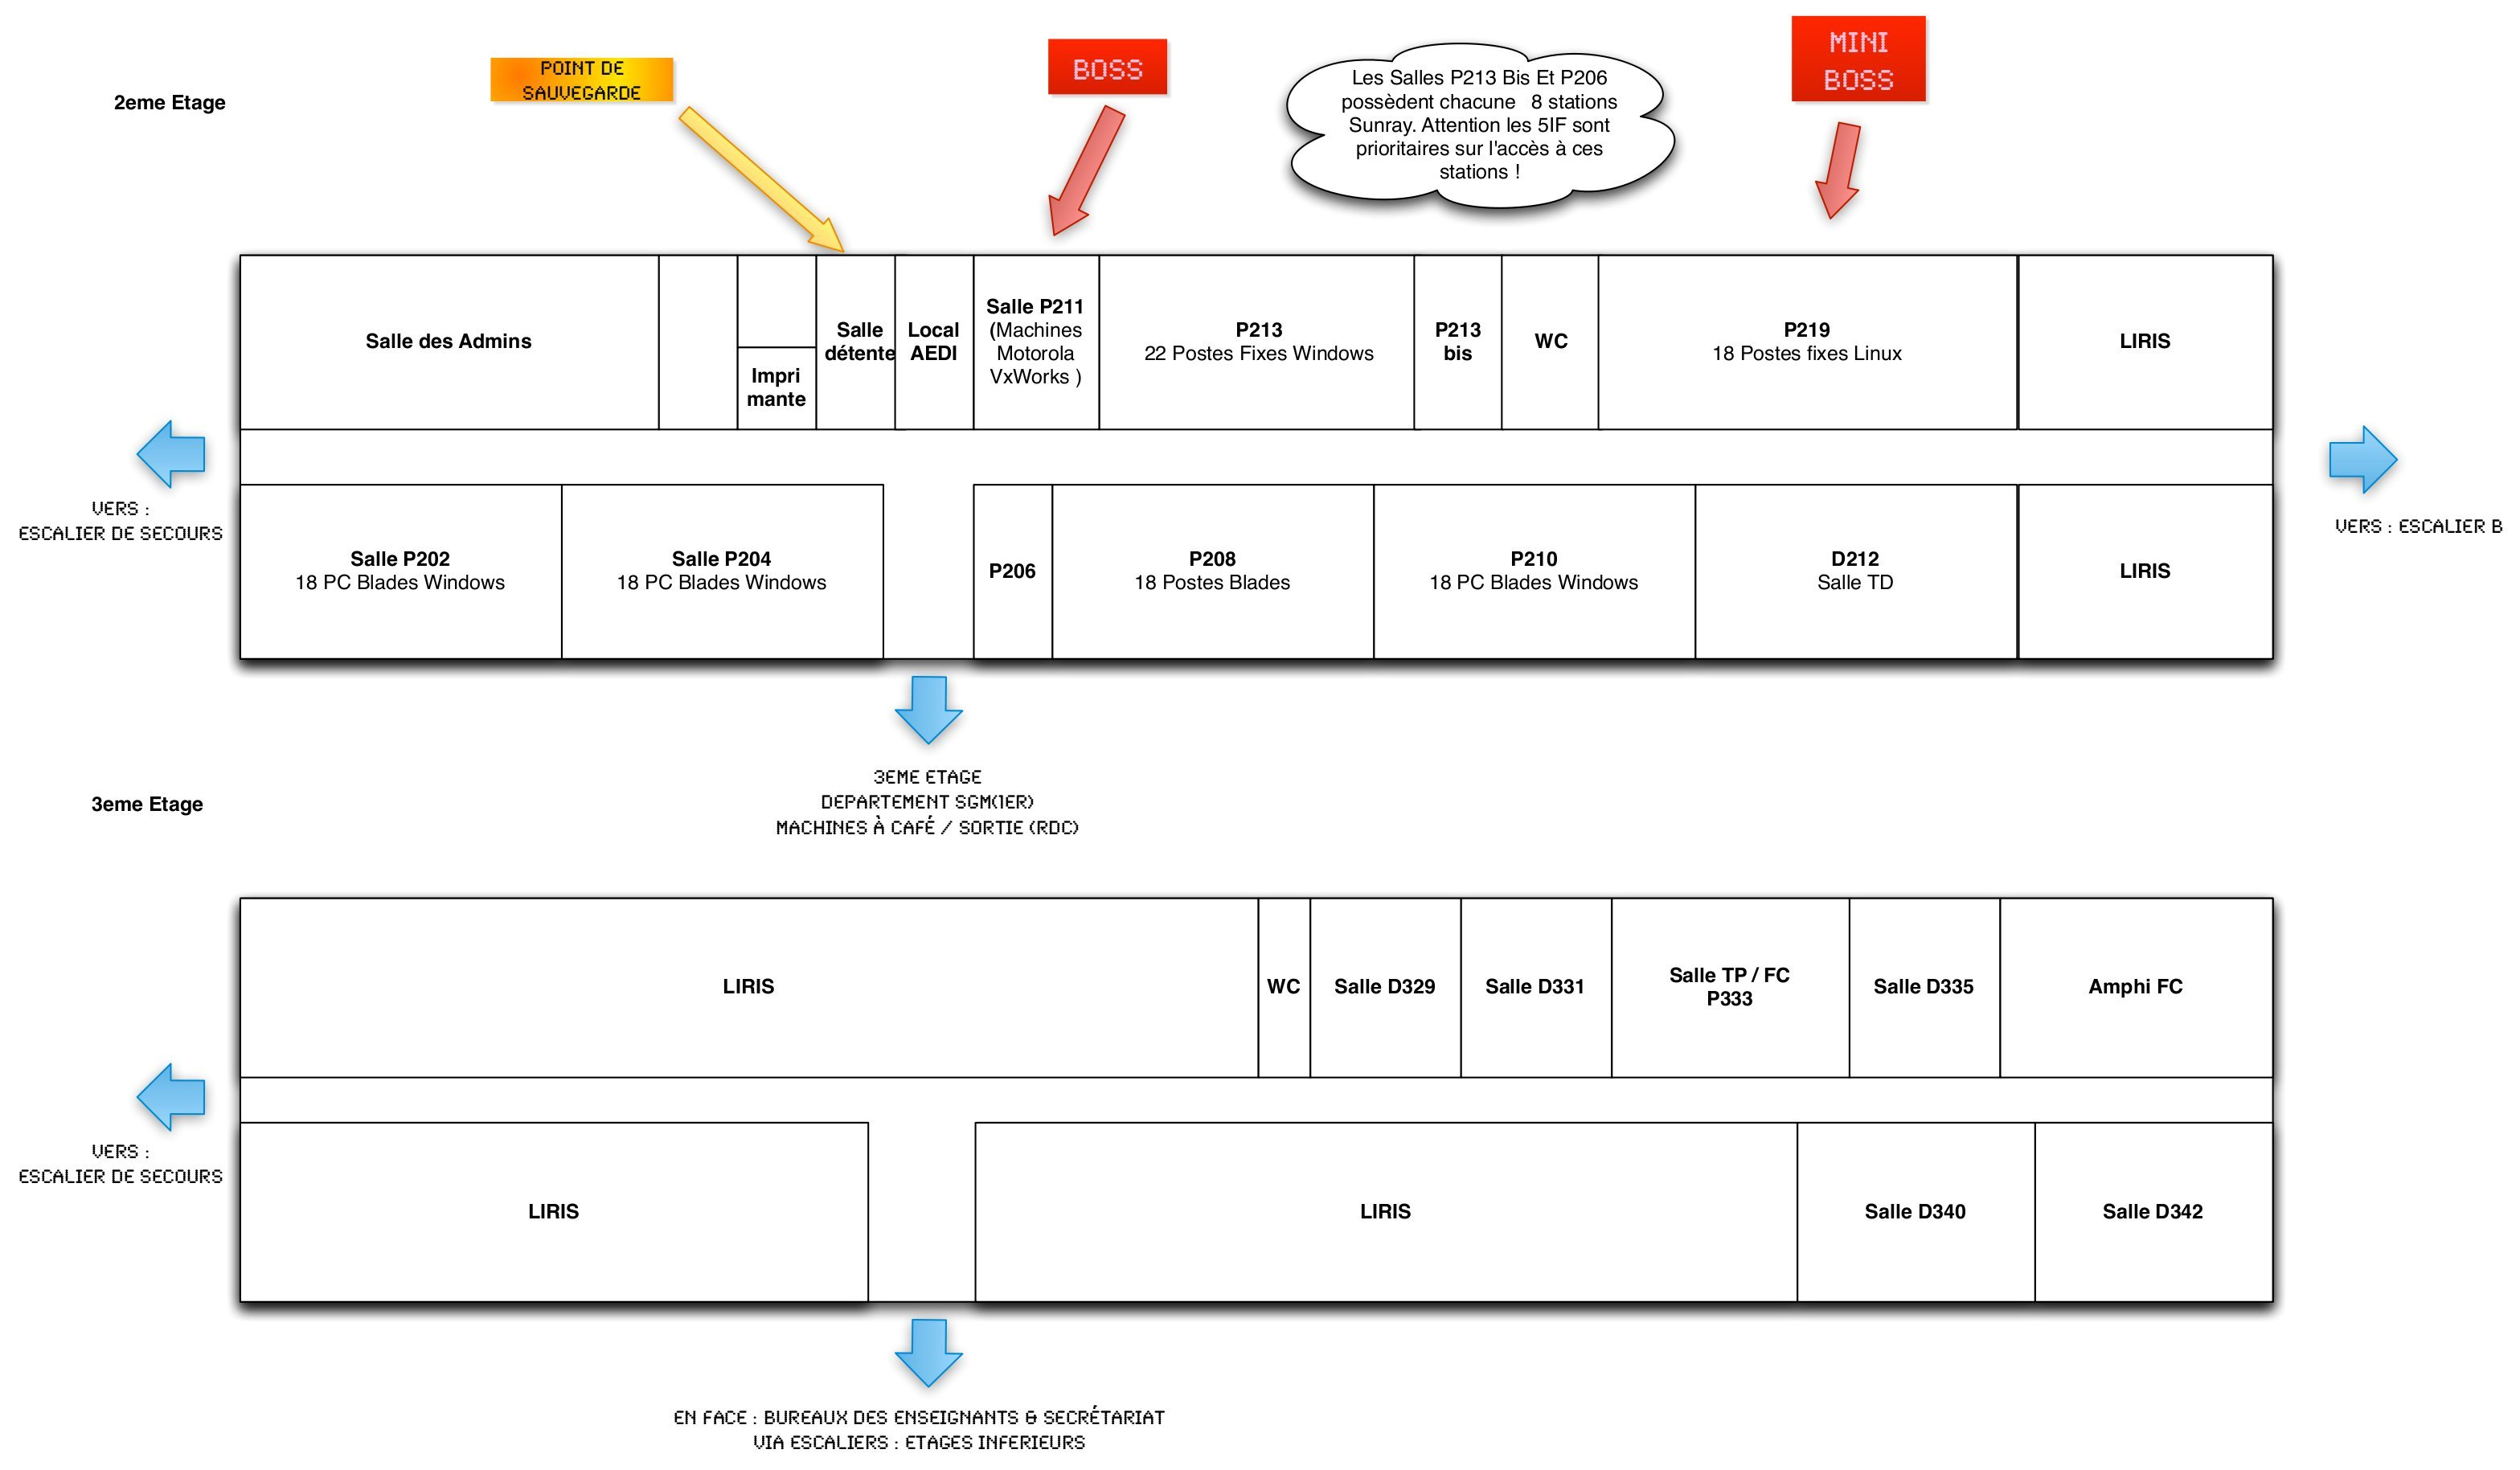
\includegraphics[width=24cm, angle=90]{images/planDepart.jpg}
\end{center}


\end{document}
